Once bin size and range are decided, we need to check if the templates 
for all signal and background processes are reasonably filled 
to avoid any biases due to poor statistics. [ref?] 

\begin{figure}[!hbtp]
	
	%
	\centering
	\subfigure[Signal]{
	\centering
	\label{subfig:template_signal_125}
		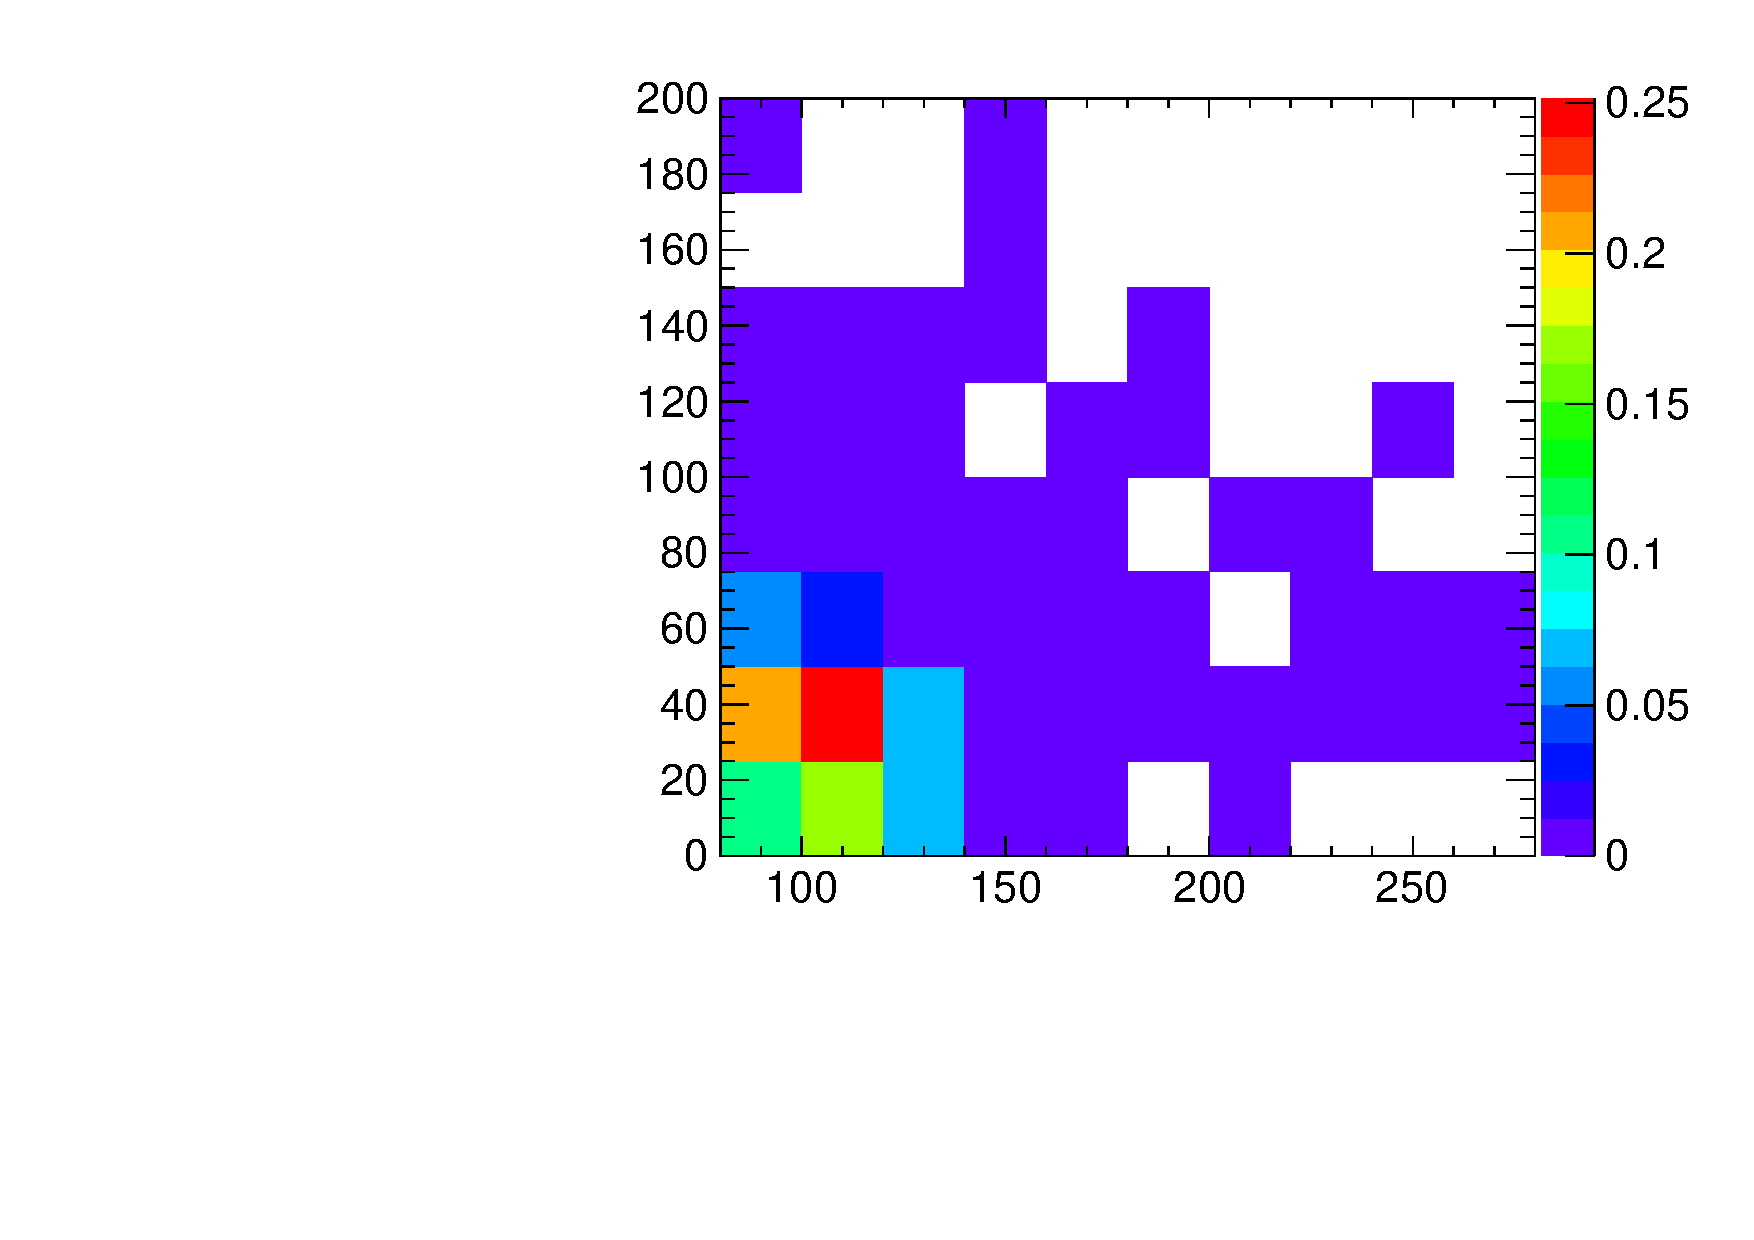
\includegraphics[width=.35\textwidth]{figures/templates/sig_2D_mH125_0j_of.pdf}
	}
	\subfigure[Signal statistical uncertainty]{
	\centering
	\label{subfig:template_signalerr_125}
		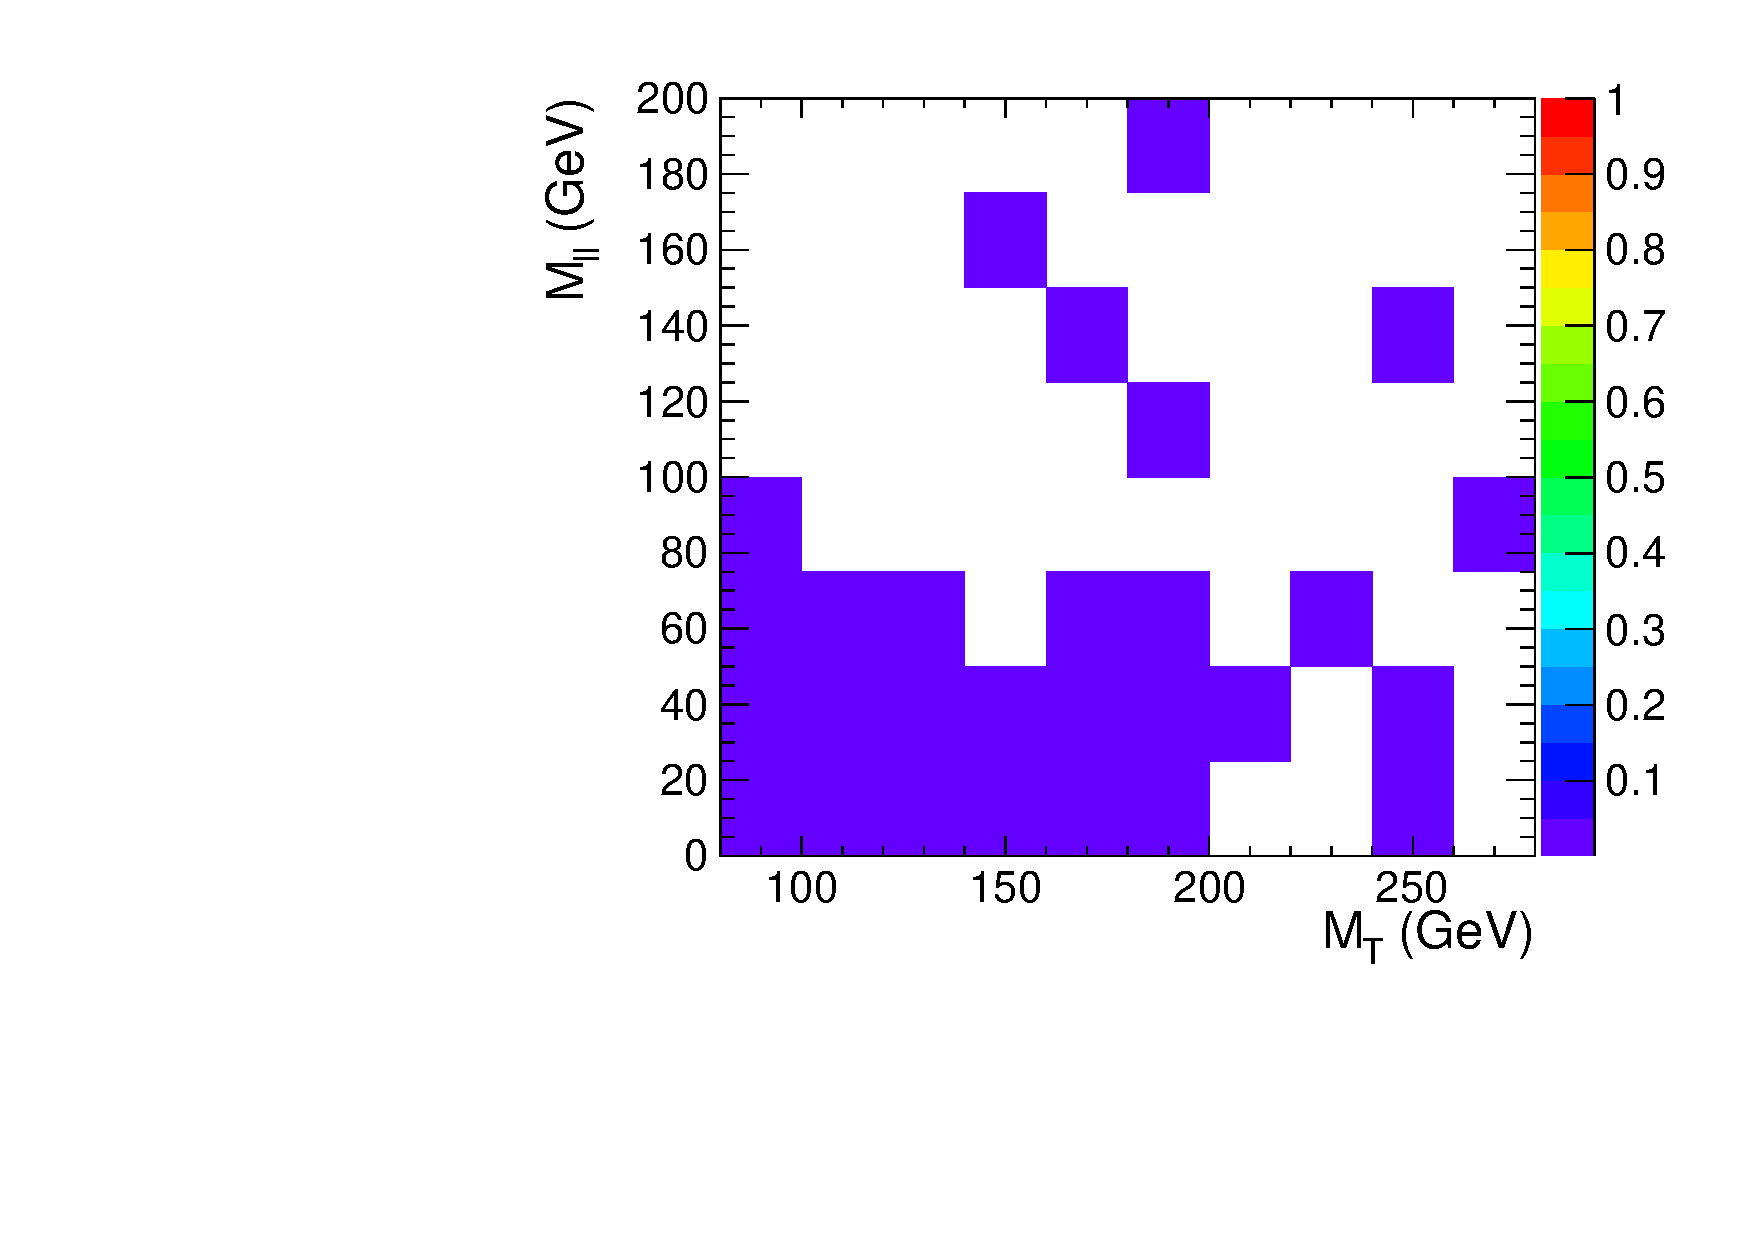
\includegraphics[width=.35\textwidth]{figures/templates/sigerr_2D_mH125_0j_of.pdf}
	}
	
	%
	\centering
	\subfigure[qqWW]{
	\centering
	\label{subfig:template_qqWW_125}
		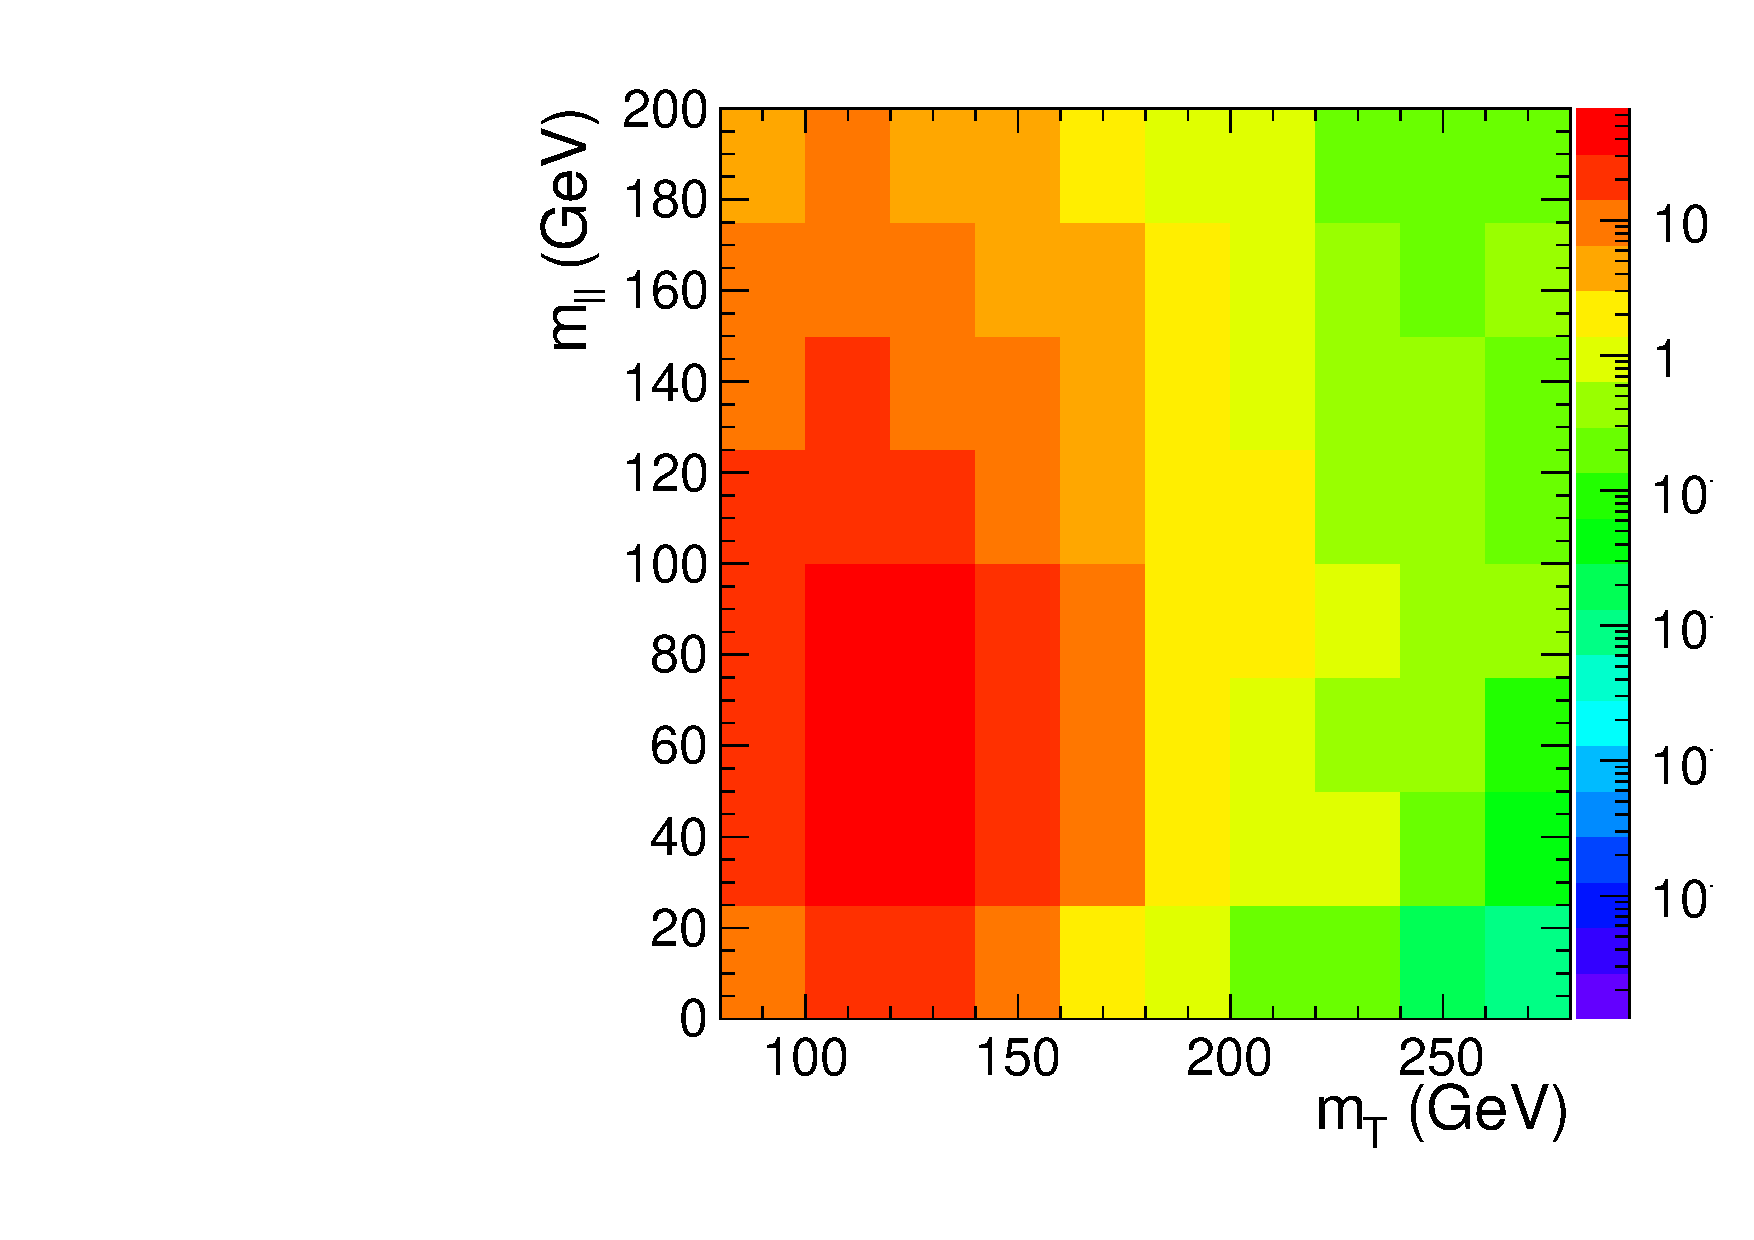
\includegraphics[width=.35\textwidth]{figures/templates/qqWW_2D_mH125_0j_of.pdf}
	}
	\subfigure[qqWW statistical uncertainty]{
	\centering
	\label{subfig:template_qqWWerr_125}
		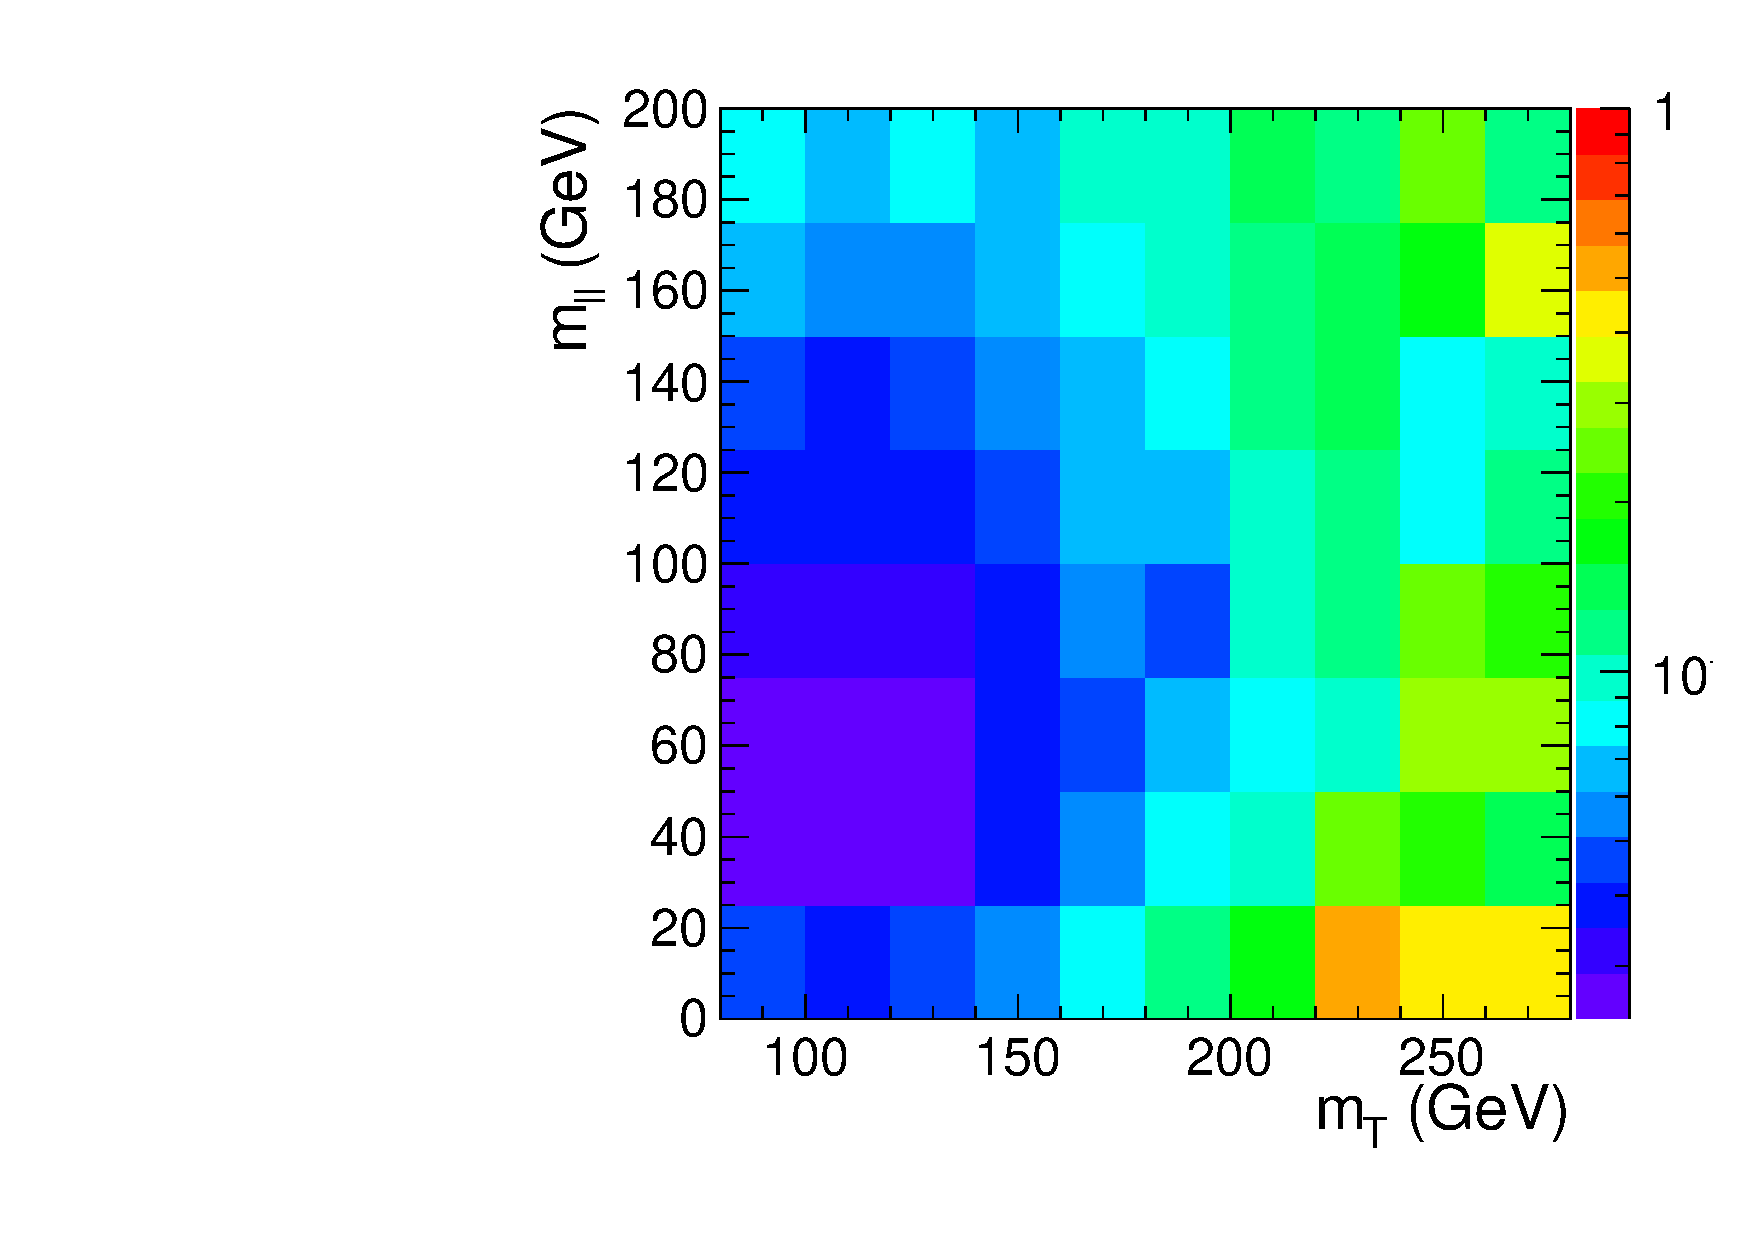
\includegraphics[width=.35\textwidth]{figures/templates/qqWWerr_2D_mH125_0j_of.pdf}
	}

	%
	\centering
	\subfigure[ggWW]{
	\centering
	\label{subfig:template_ggWW_125}
		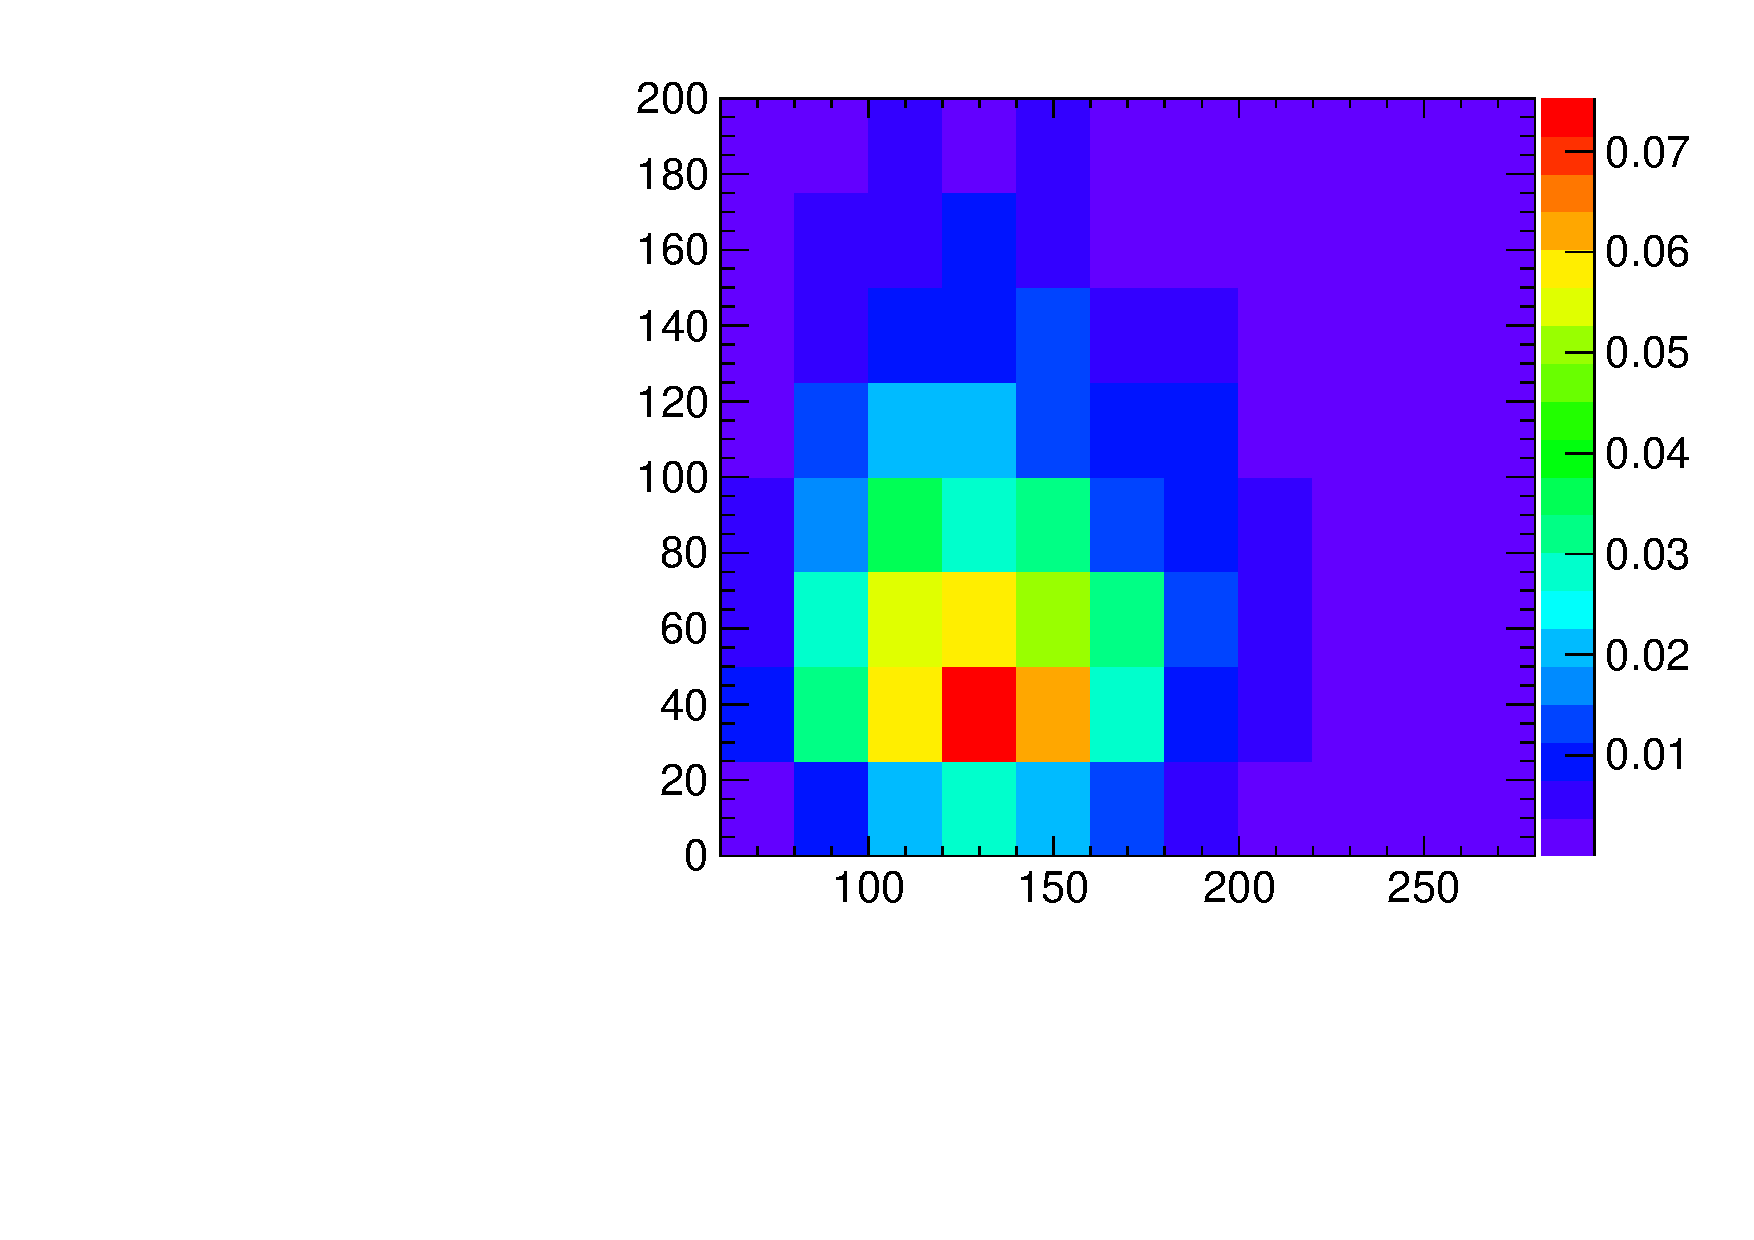
\includegraphics[width=.35\textwidth]{figures/templates/ggWW_2D_mH125_0j_of.pdf}
	}
	\subfigure[ggWW statistical uncertainty]{
	\centering
	\label{subfig:template_ggWWerr_125}
		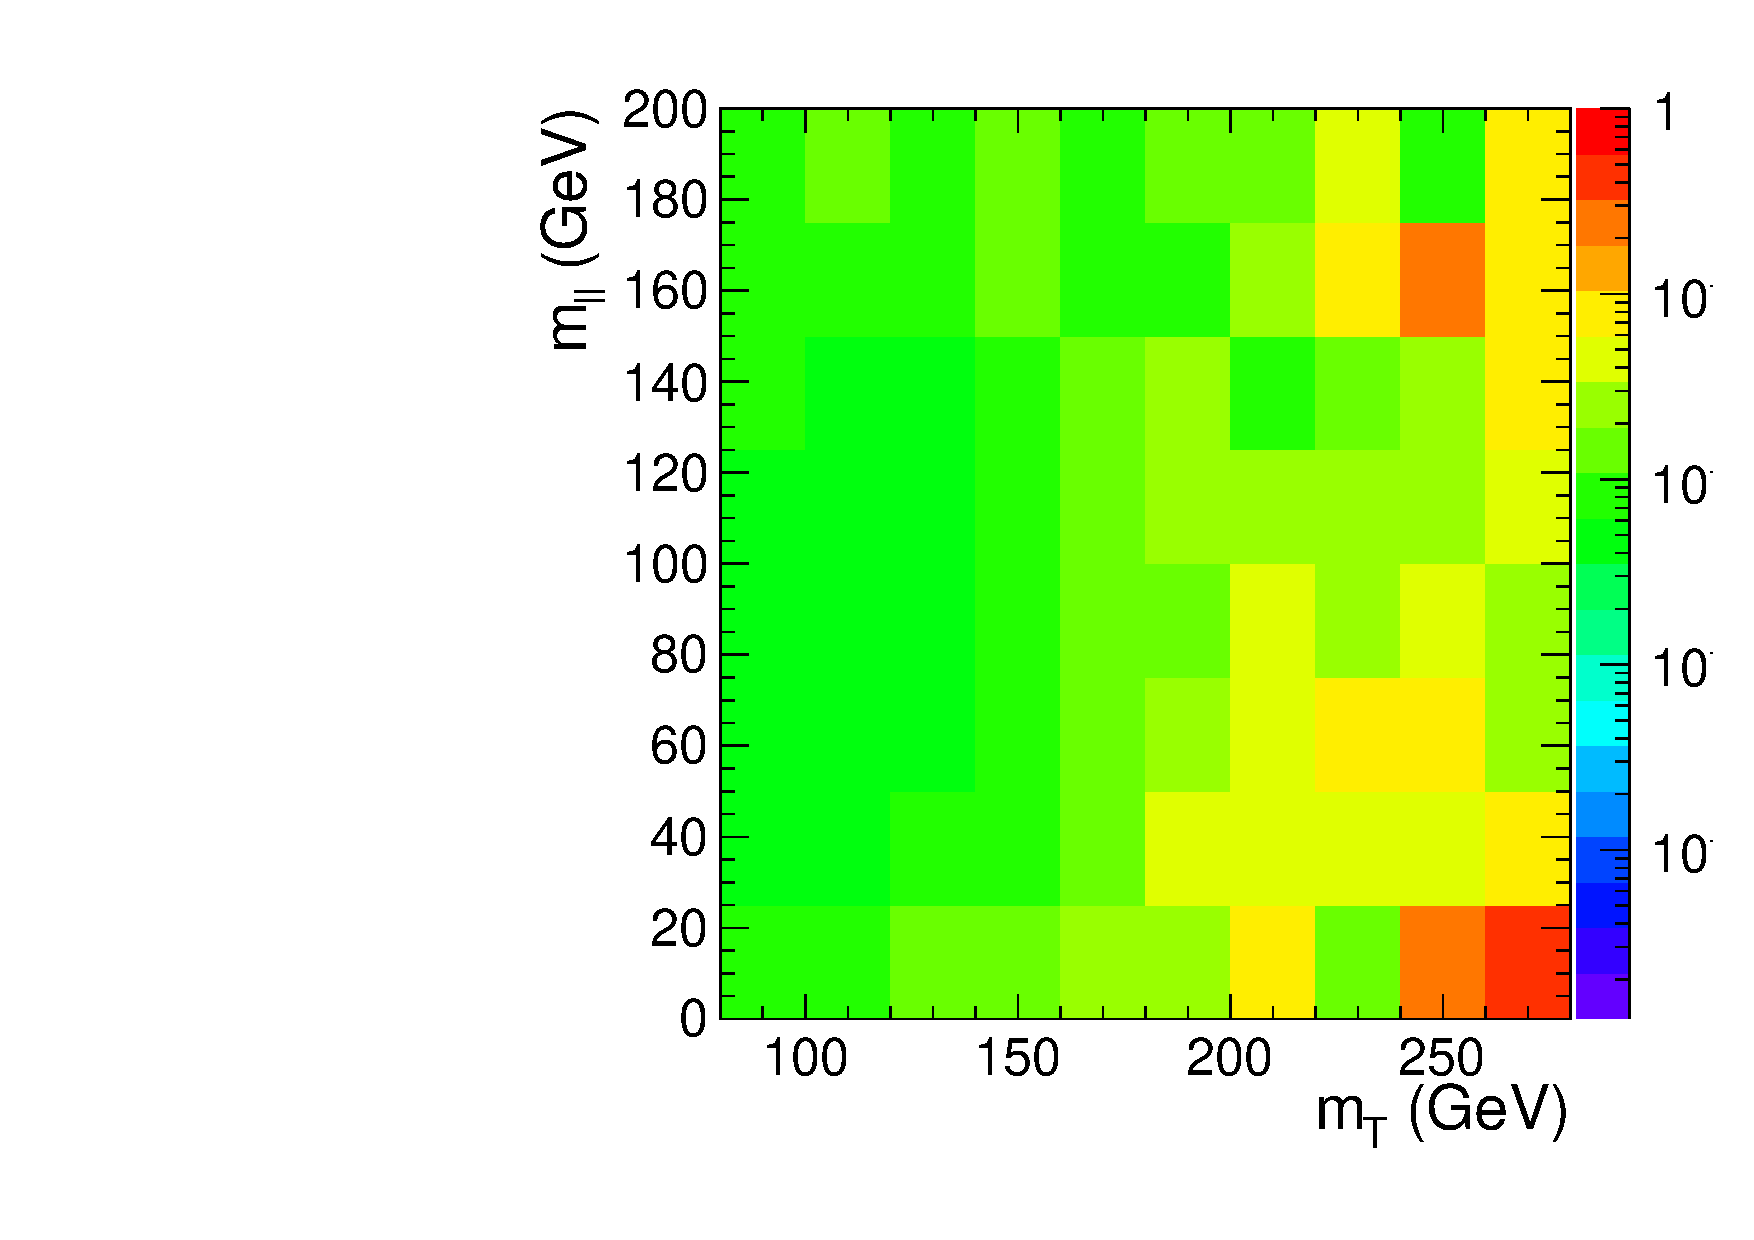
\includegraphics[width=.35\textwidth]{figures/templates/ggWWerr_2D_mH125_0j_of.pdf}
	}

	\caption{2D templates at \mHi = 125 \GeV} 
	\label{fig:templates_125_1}

\end{figure}

\begin{figure}[!hbtp]
	
	%
	\centering
	\subfigure[Wjets]{
	\centering
	\label{subfig:template_Wjets_125}
		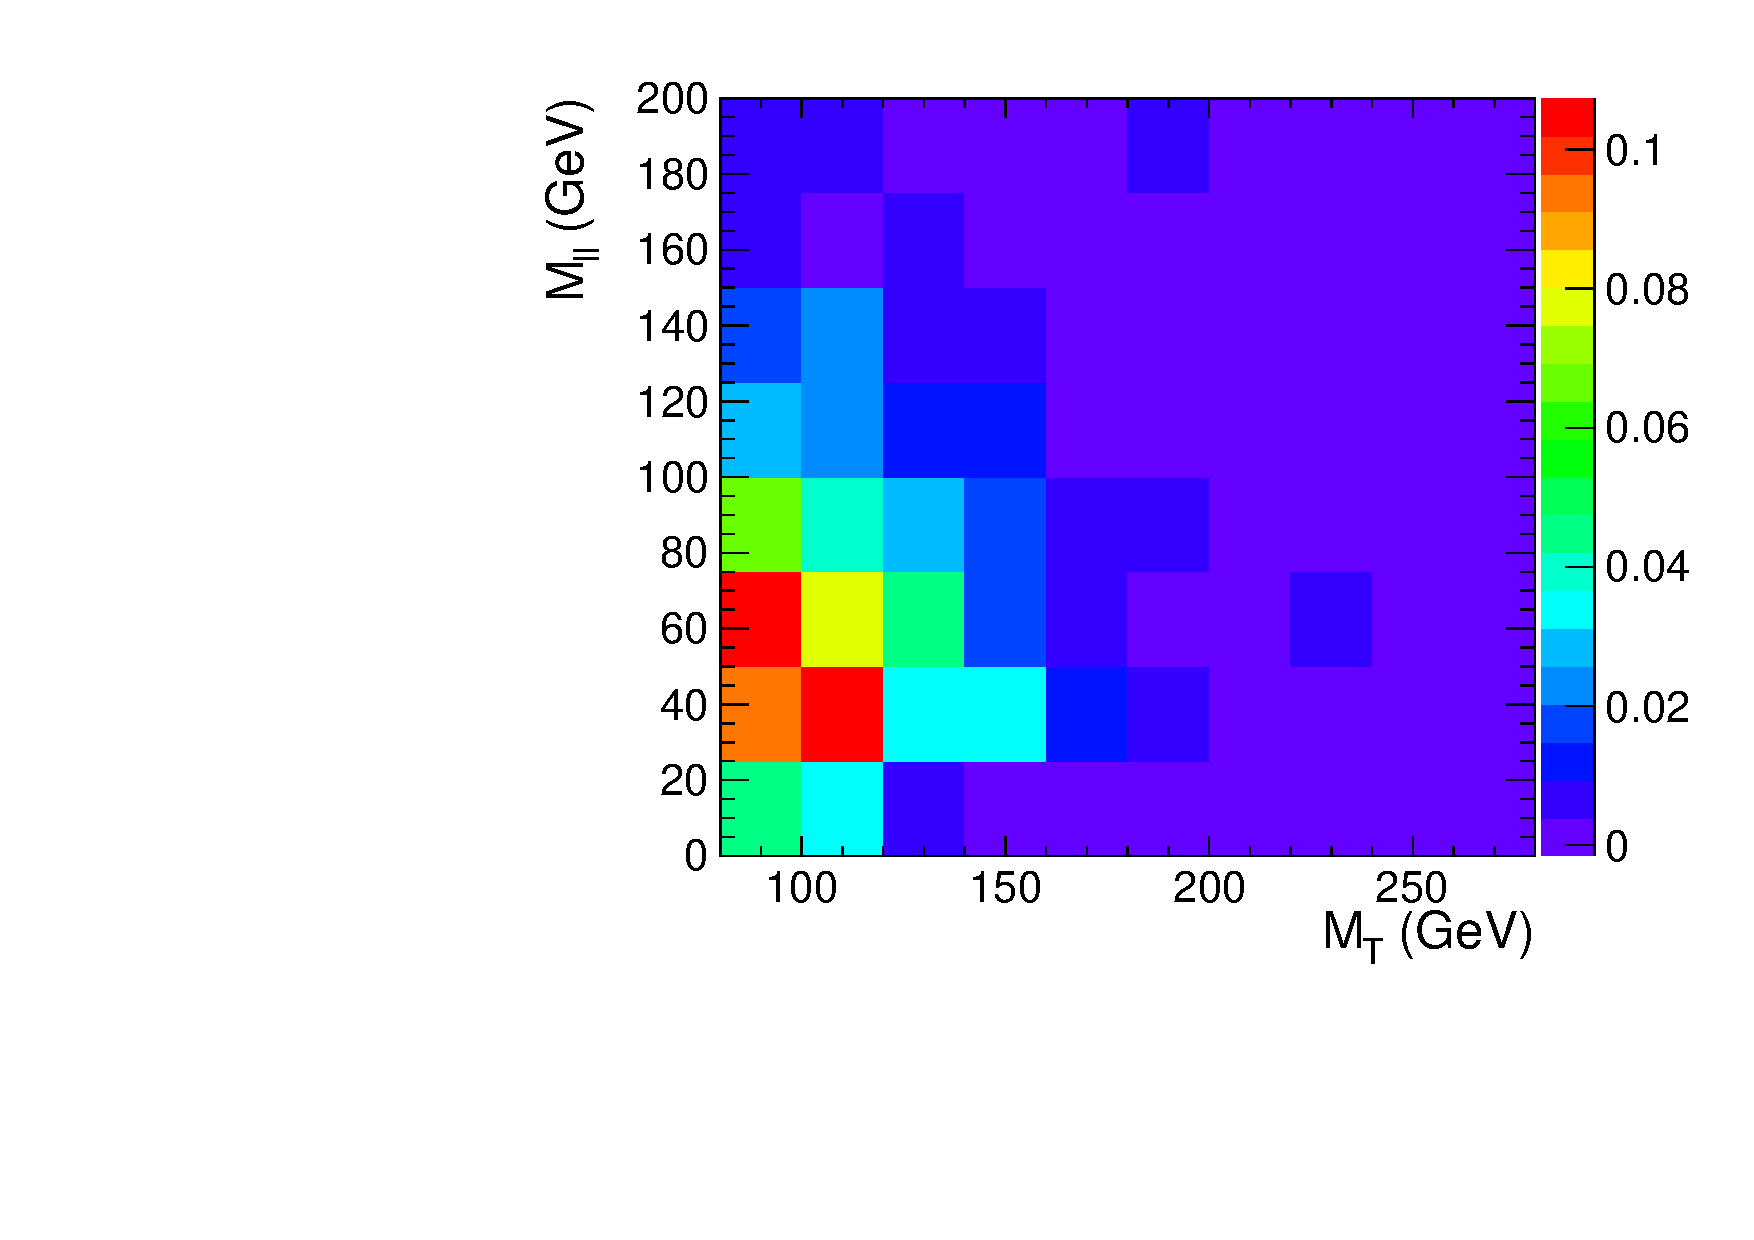
\includegraphics[width=.35\textwidth]{figures/templates/Wjets_2D_mH125_0j_of.pdf}
	}
	\subfigure[Wjets statistical uncertainty]{
	\centering
	\label{subfig:template_Wjetserr_125}
		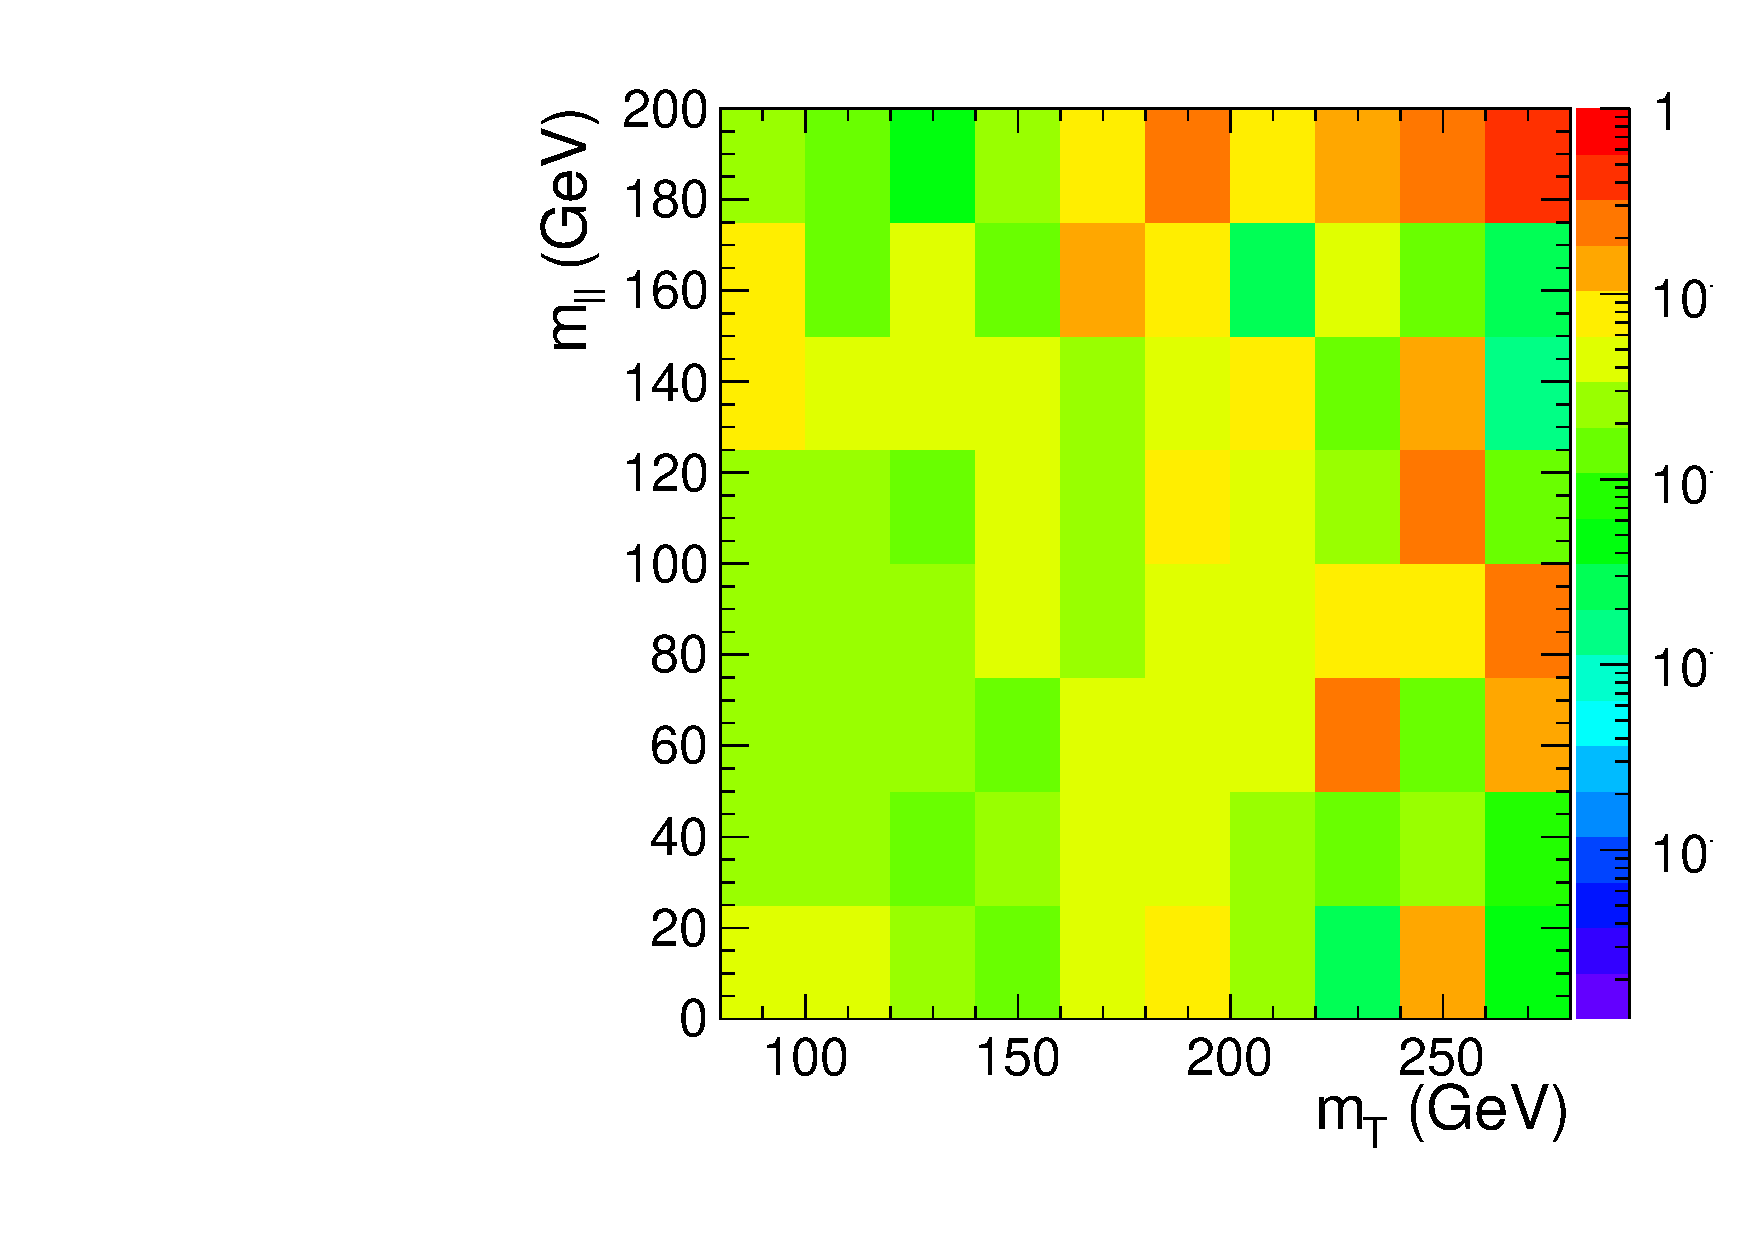
\includegraphics[width=.35\textwidth]{figures/templates/Wjetserr_2D_mH125_0j_of.pdf}
	}
	
	%
	\centering
	\subfigure[Top]{
	\centering
	\label{subfig:template_Top_125}
		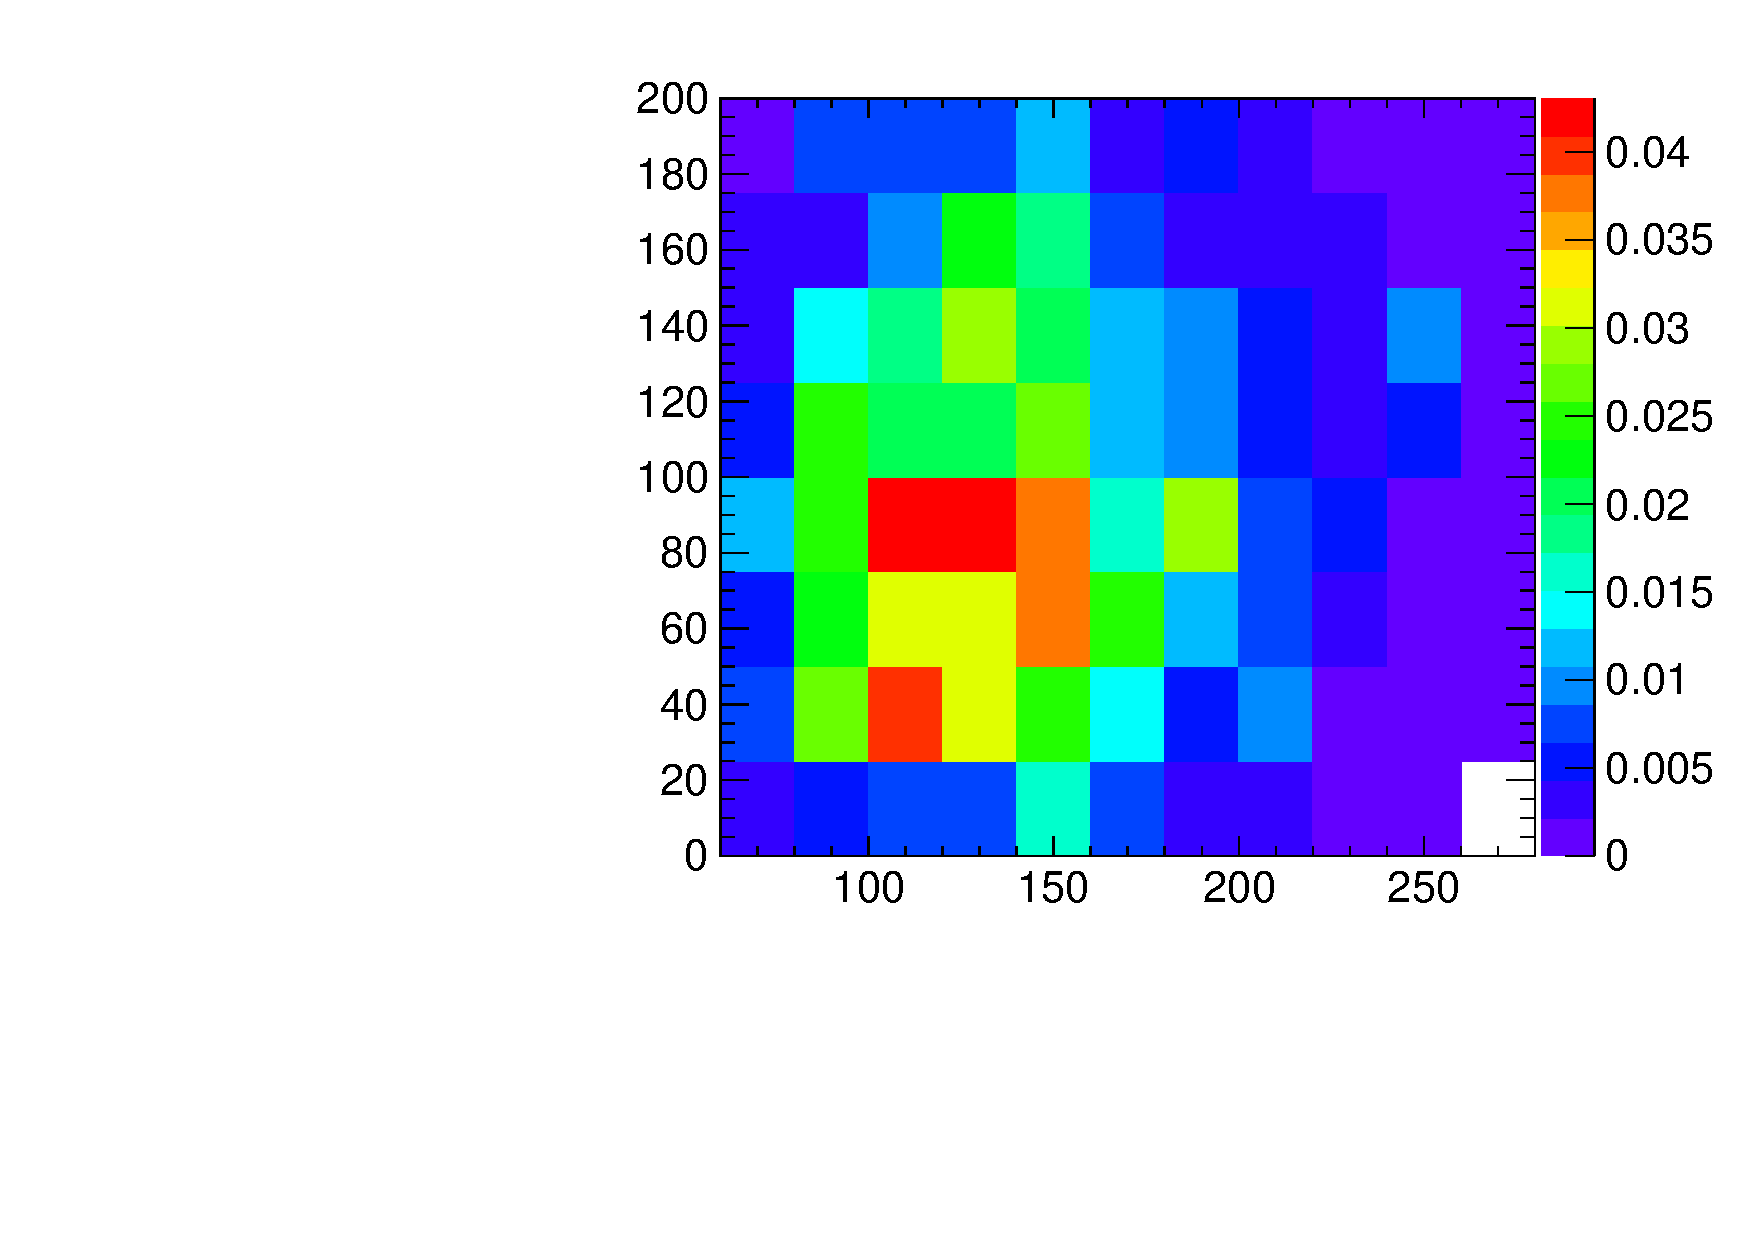
\includegraphics[width=.35\textwidth]{figures/templates/Top_2D_mH125_0j_of.pdf}
	}
	\subfigure[Top statistical uncertainty]{
	\centering
	\label{subfig:template_Toperr_125}
		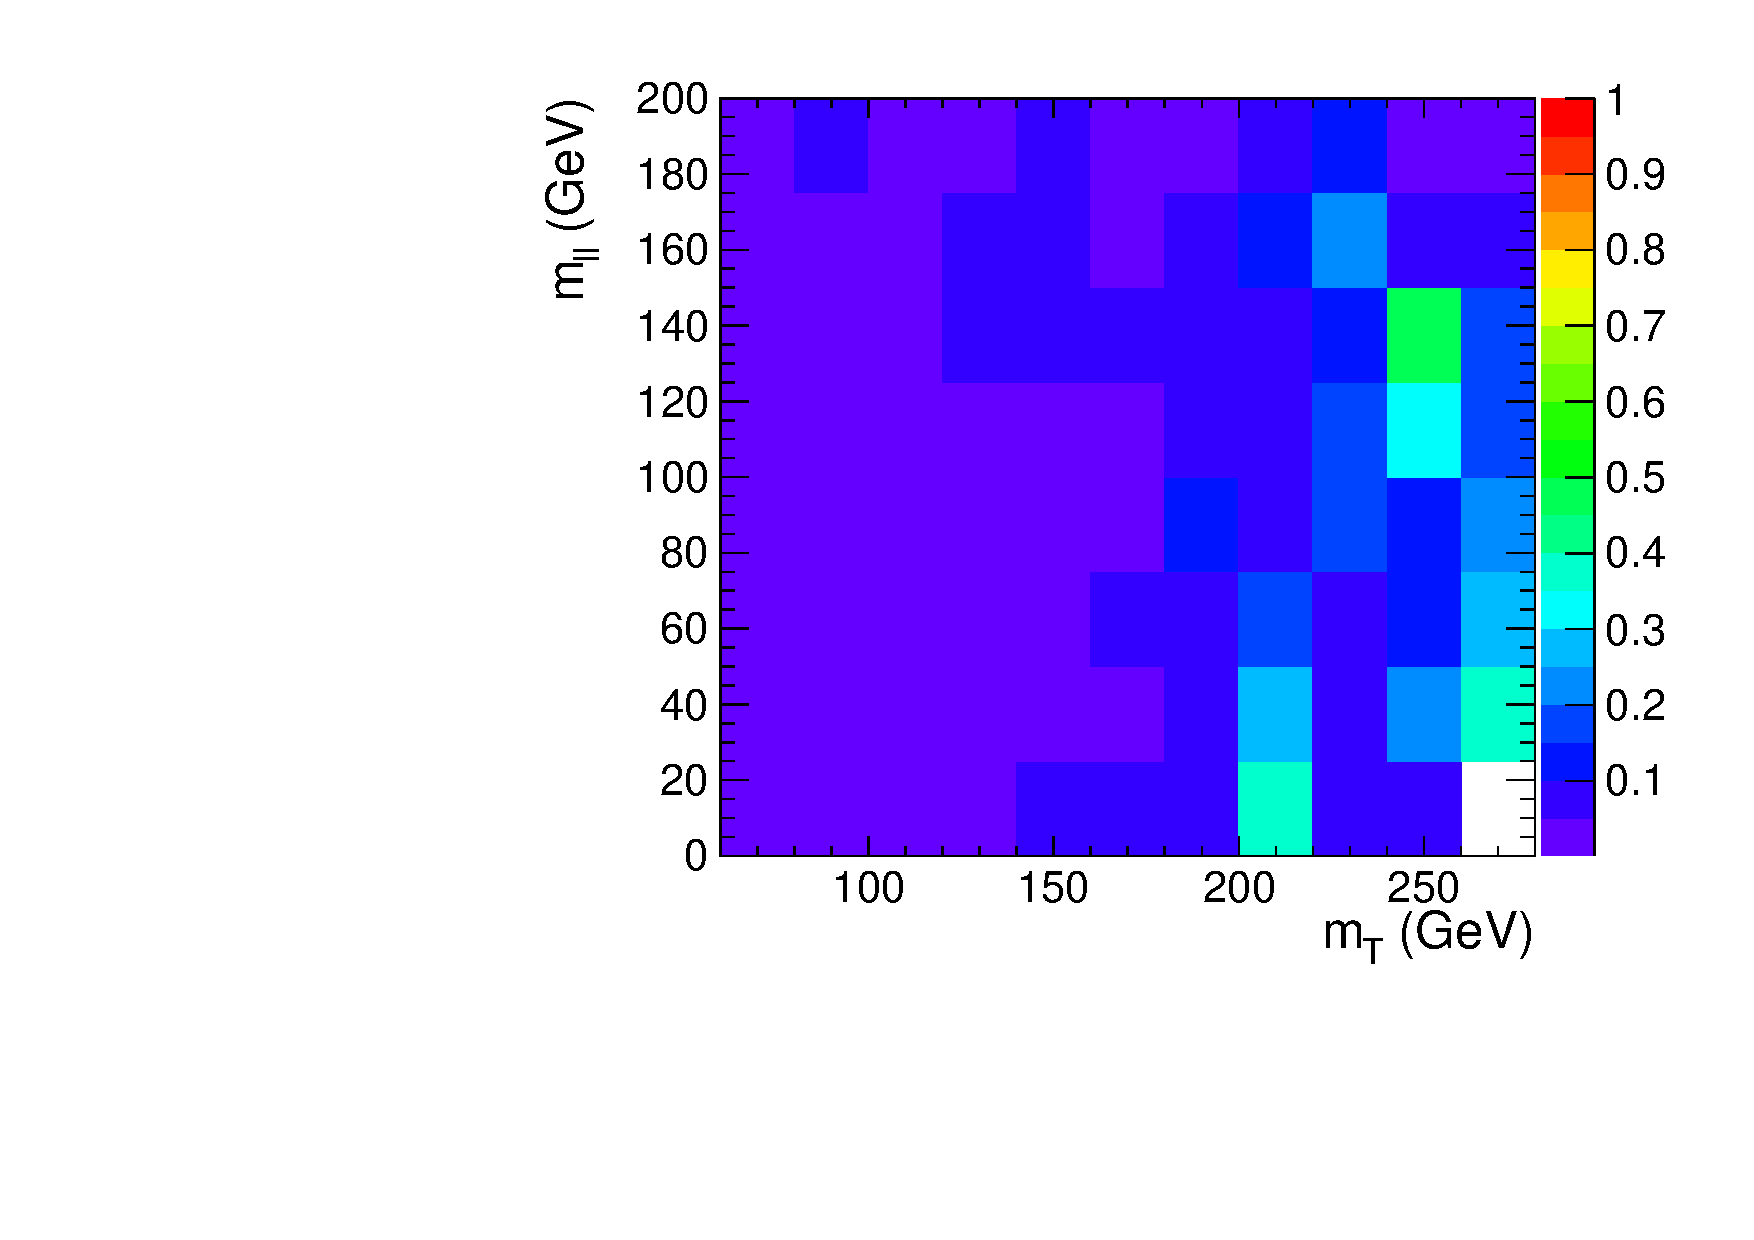
\includegraphics[width=.35\textwidth]{figures/templates/Toperr_2D_mH125_0j_of.pdf}
	}

	%
	\centering
	\subfigure[VV]{
	\centering
	\label{subfig:template_VV_125}
		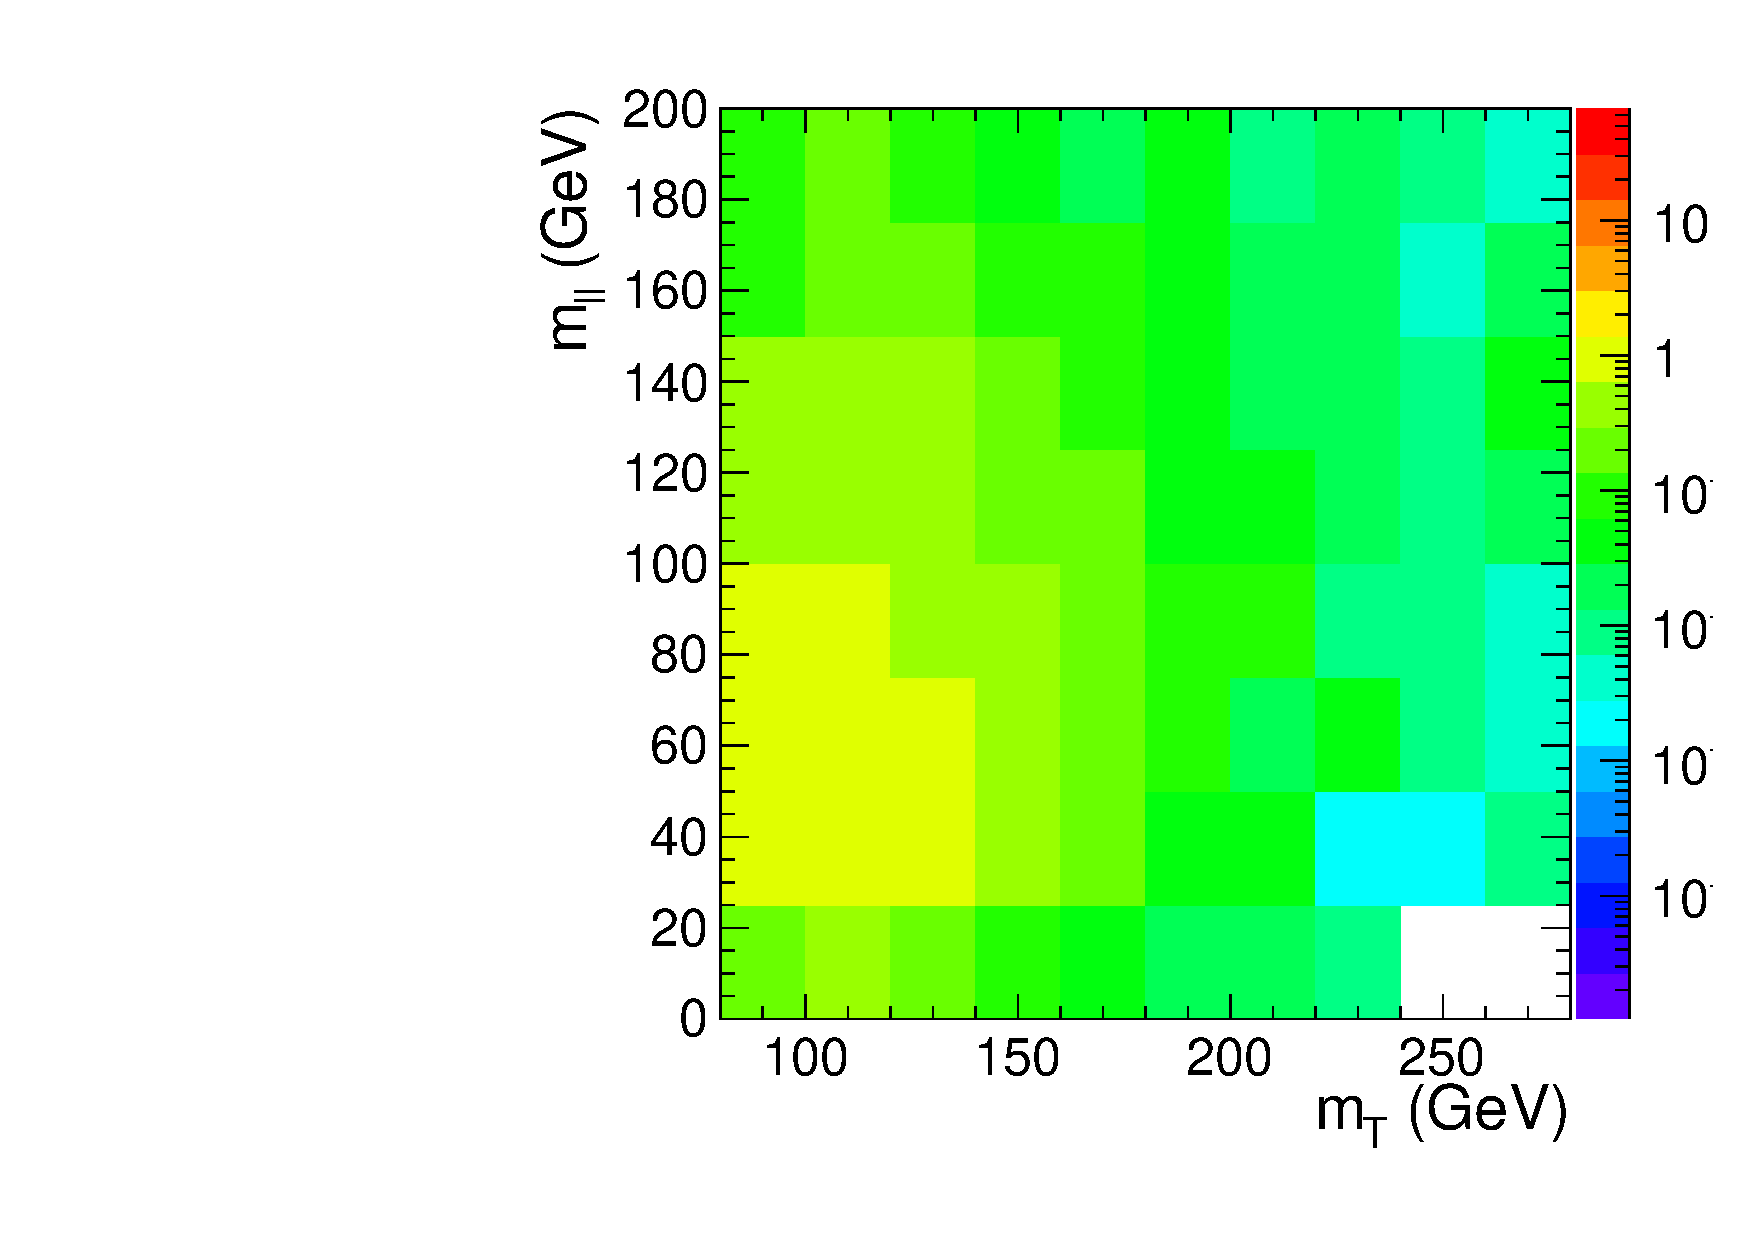
\includegraphics[width=.35\textwidth]{figures/templates/VV_2D_mH125_0j_of.pdf}
	}
	\subfigure[VV statistical uncertainty]{
	\centering
	\label{subfig:template_VVerr_125}
		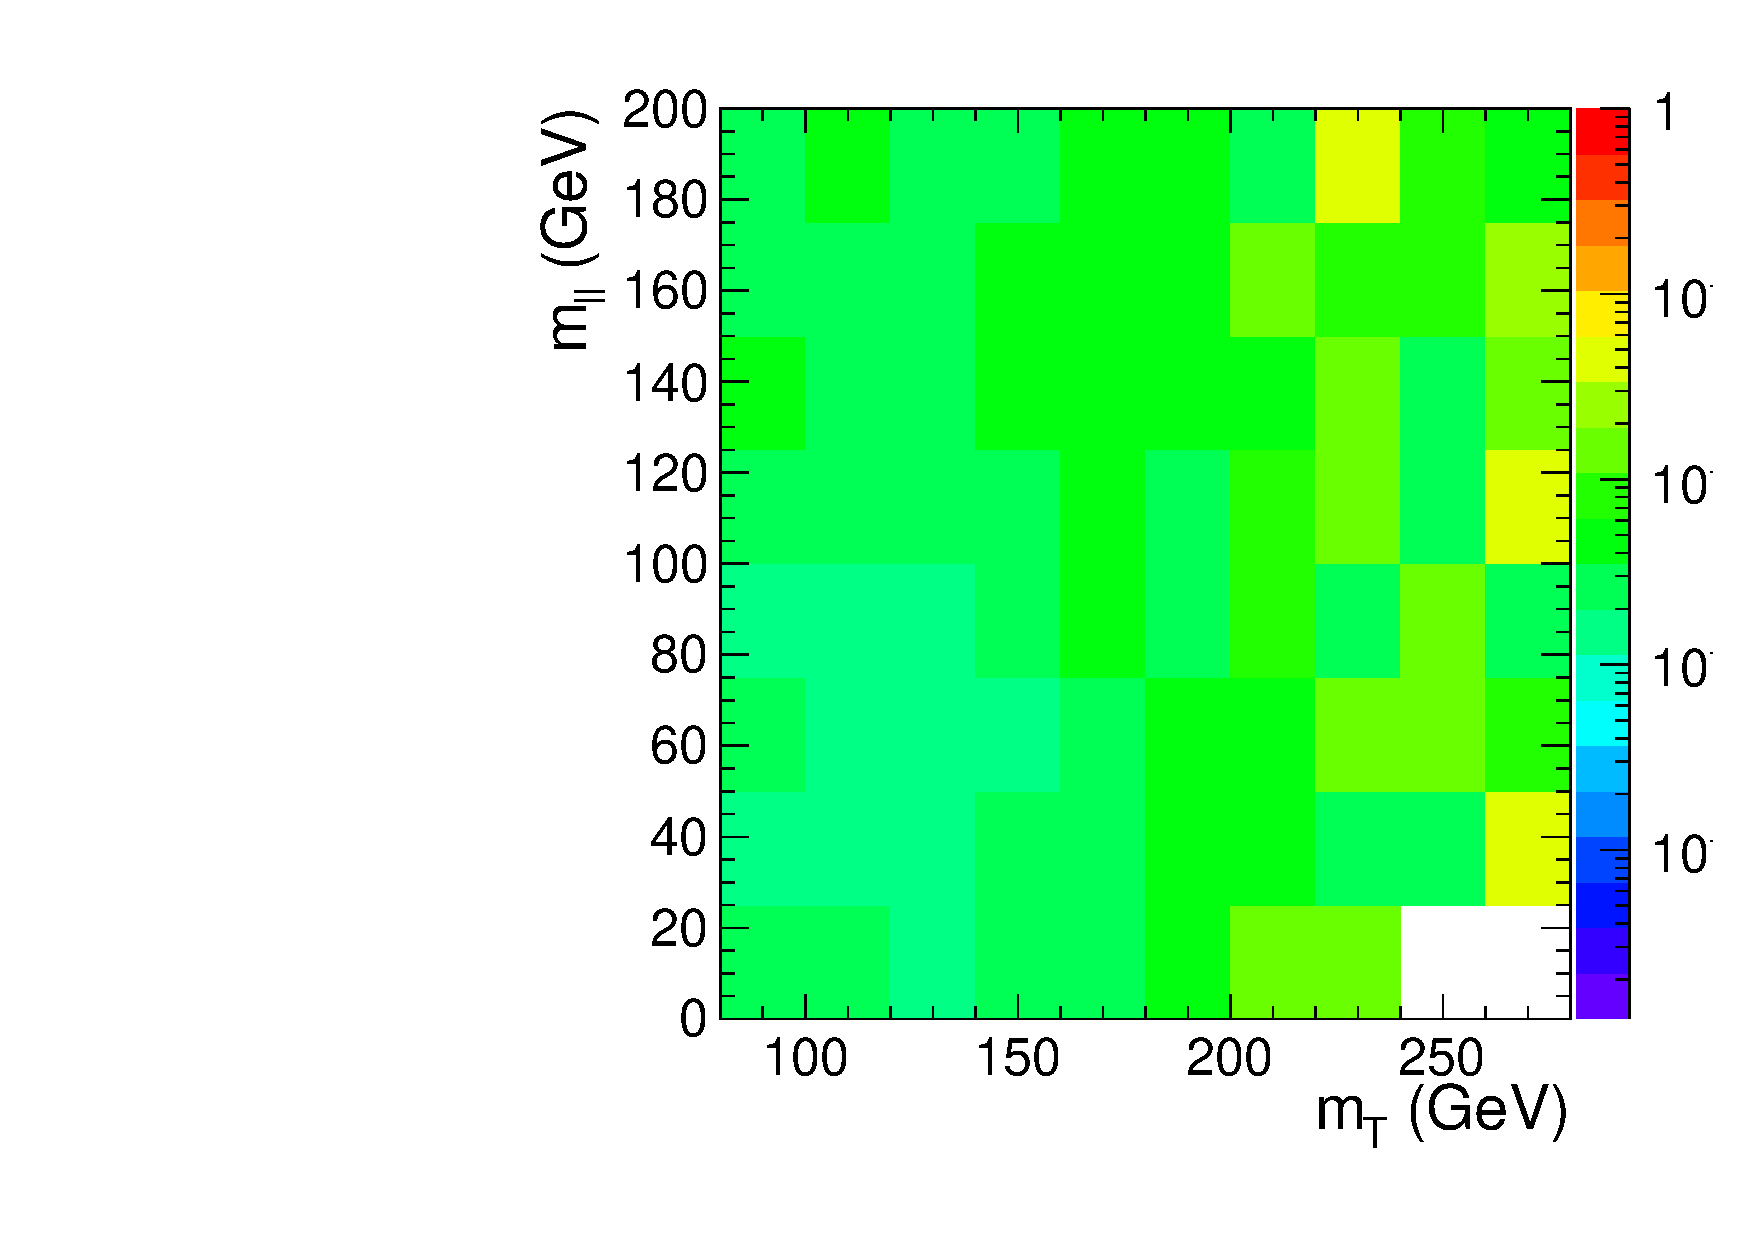
\includegraphics[width=.35\textwidth]{figures/templates/VVerr_2D_mH125_0j_of.pdf}
	}

	\caption{2D templates at \mHi = 125 \GeV} 
	\label{fig:templates_125_2}

\end{figure}

\begin{figure}[!hbtp]
	
	%
	\centering
	\subfigure[Zjets]{
	\centering
	\label{subfig:template_Zjets_125}
		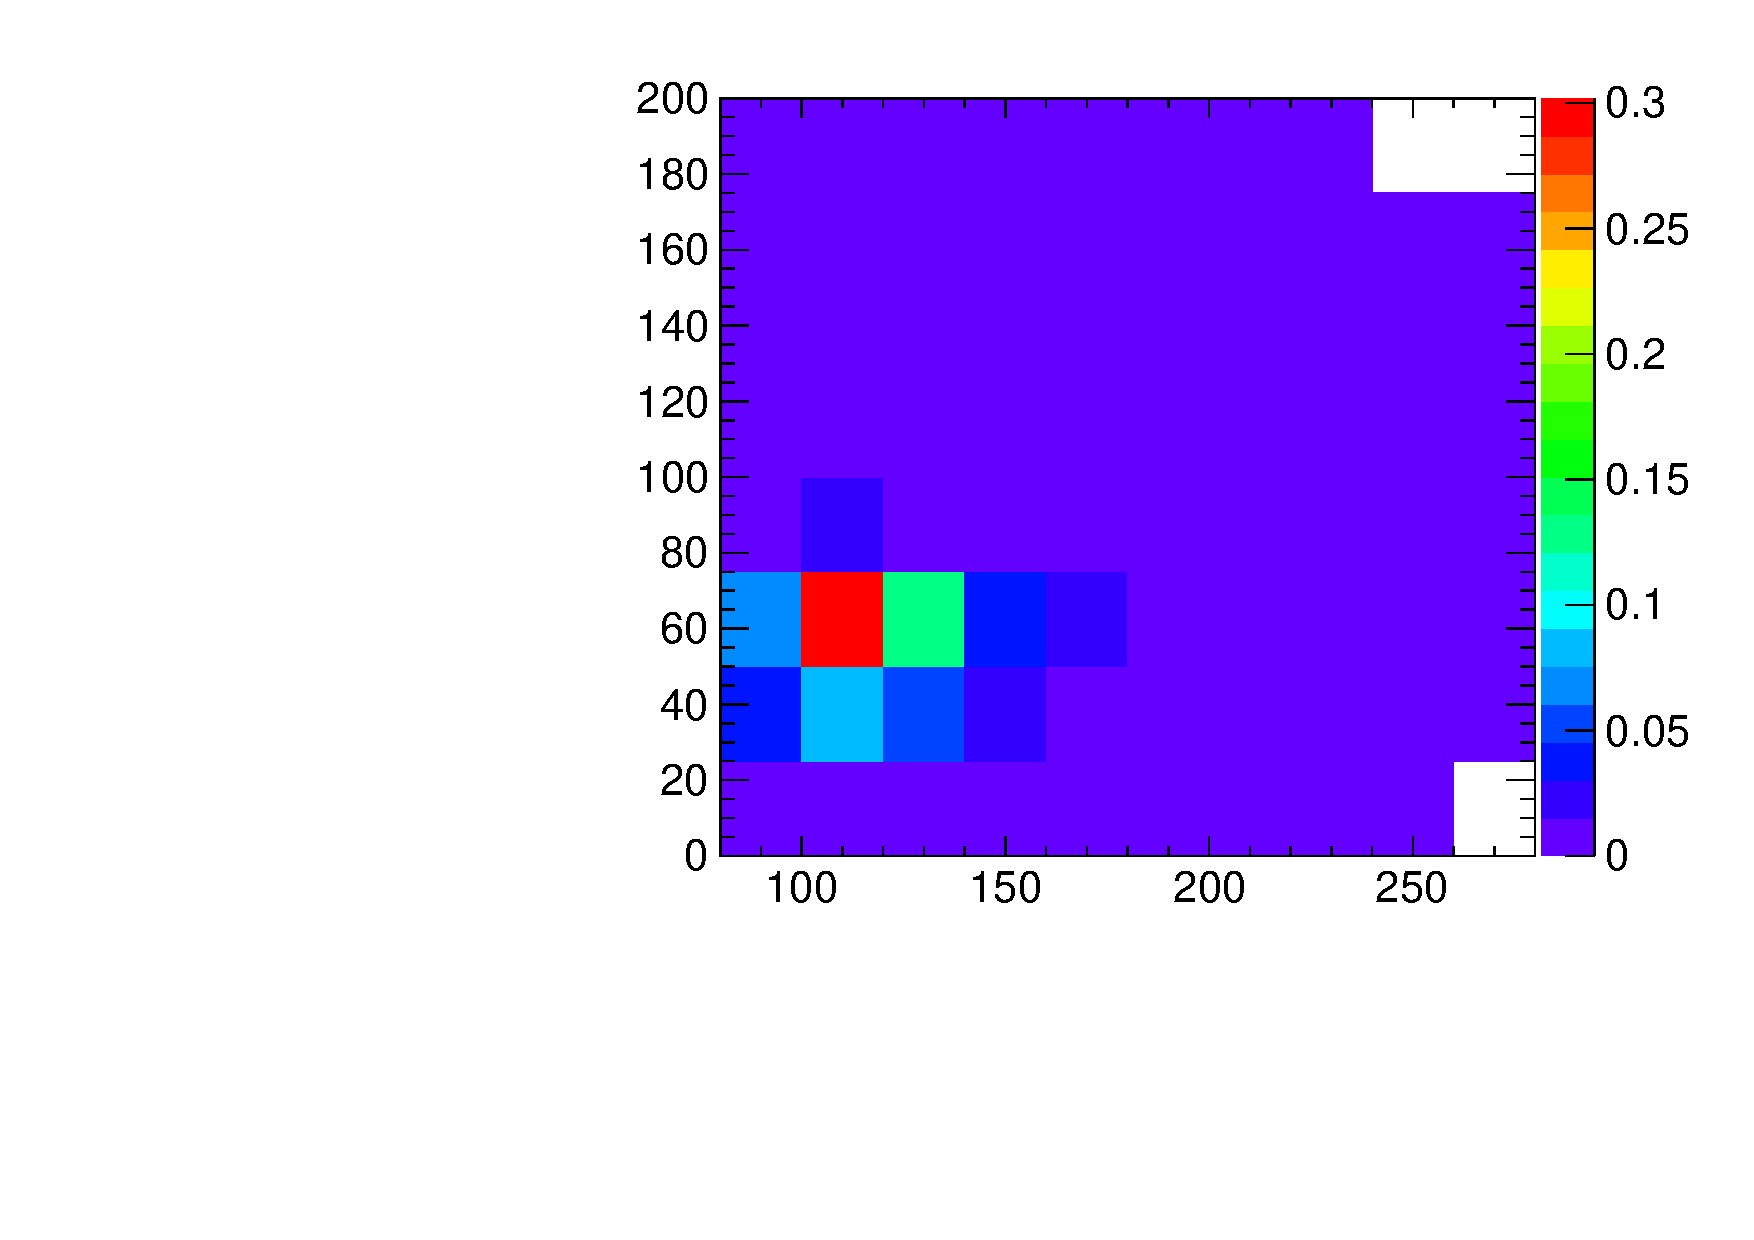
\includegraphics[width=.35\textwidth]{figures/templates/Zjets_2D_mH125_0j_of.pdf}
	}
	\subfigure[Zjets statistical uncertainty]{
	\centering
	\label{subfig:template_Zjetserr_125}
		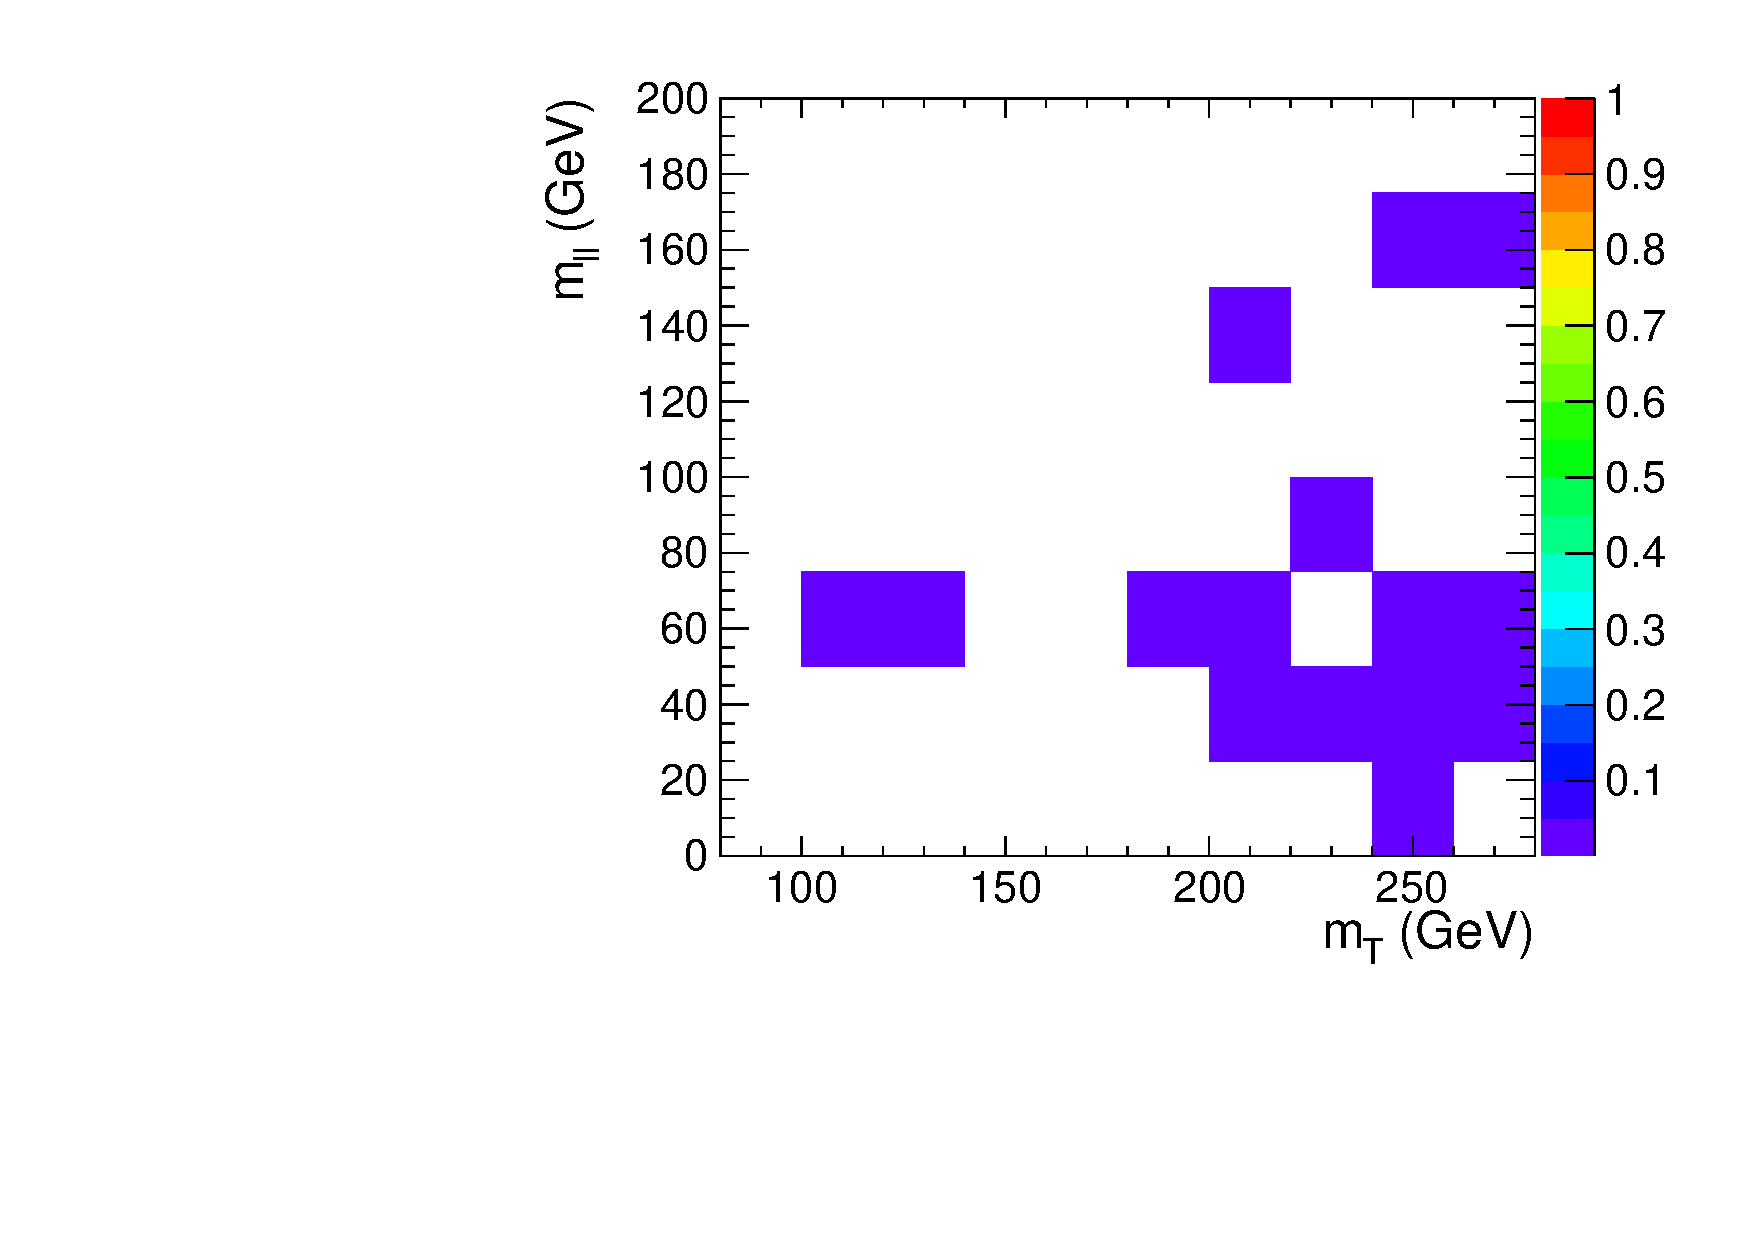
\includegraphics[width=.35\textwidth]{figures/templates/Zjetserr_2D_mH125_0j_of.pdf}
	}

	%
	\centering
	\subfigure[Wgamma]{
	\centering
	\label{subfig:template_Wgamma_125}
		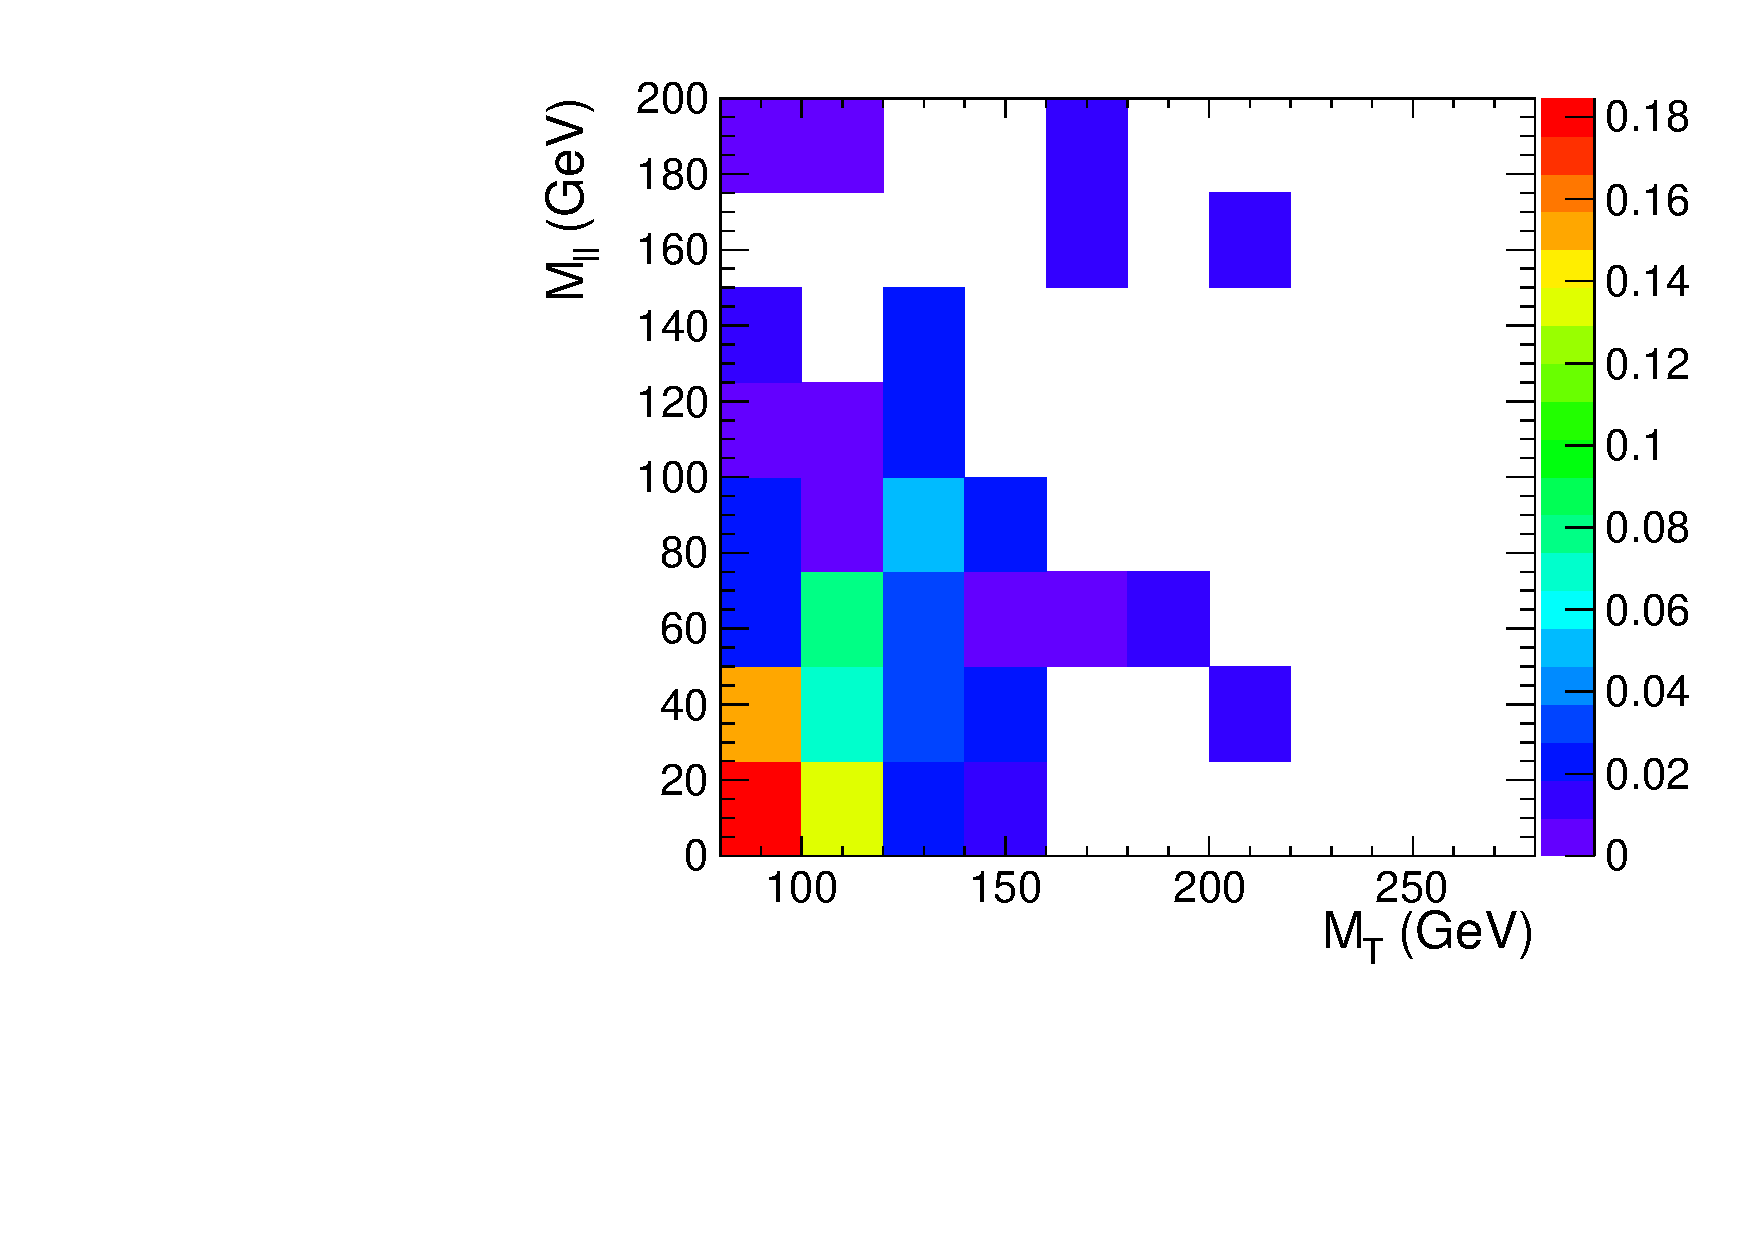
\includegraphics[width=.35\textwidth]{figures/templates/Wgamma_2D_mH125_0j_of.pdf}
	}
	\subfigure[Wgamma statistical uncertainty]{
	\centering
	\label{subfig:template_Wgammaerr_125}
		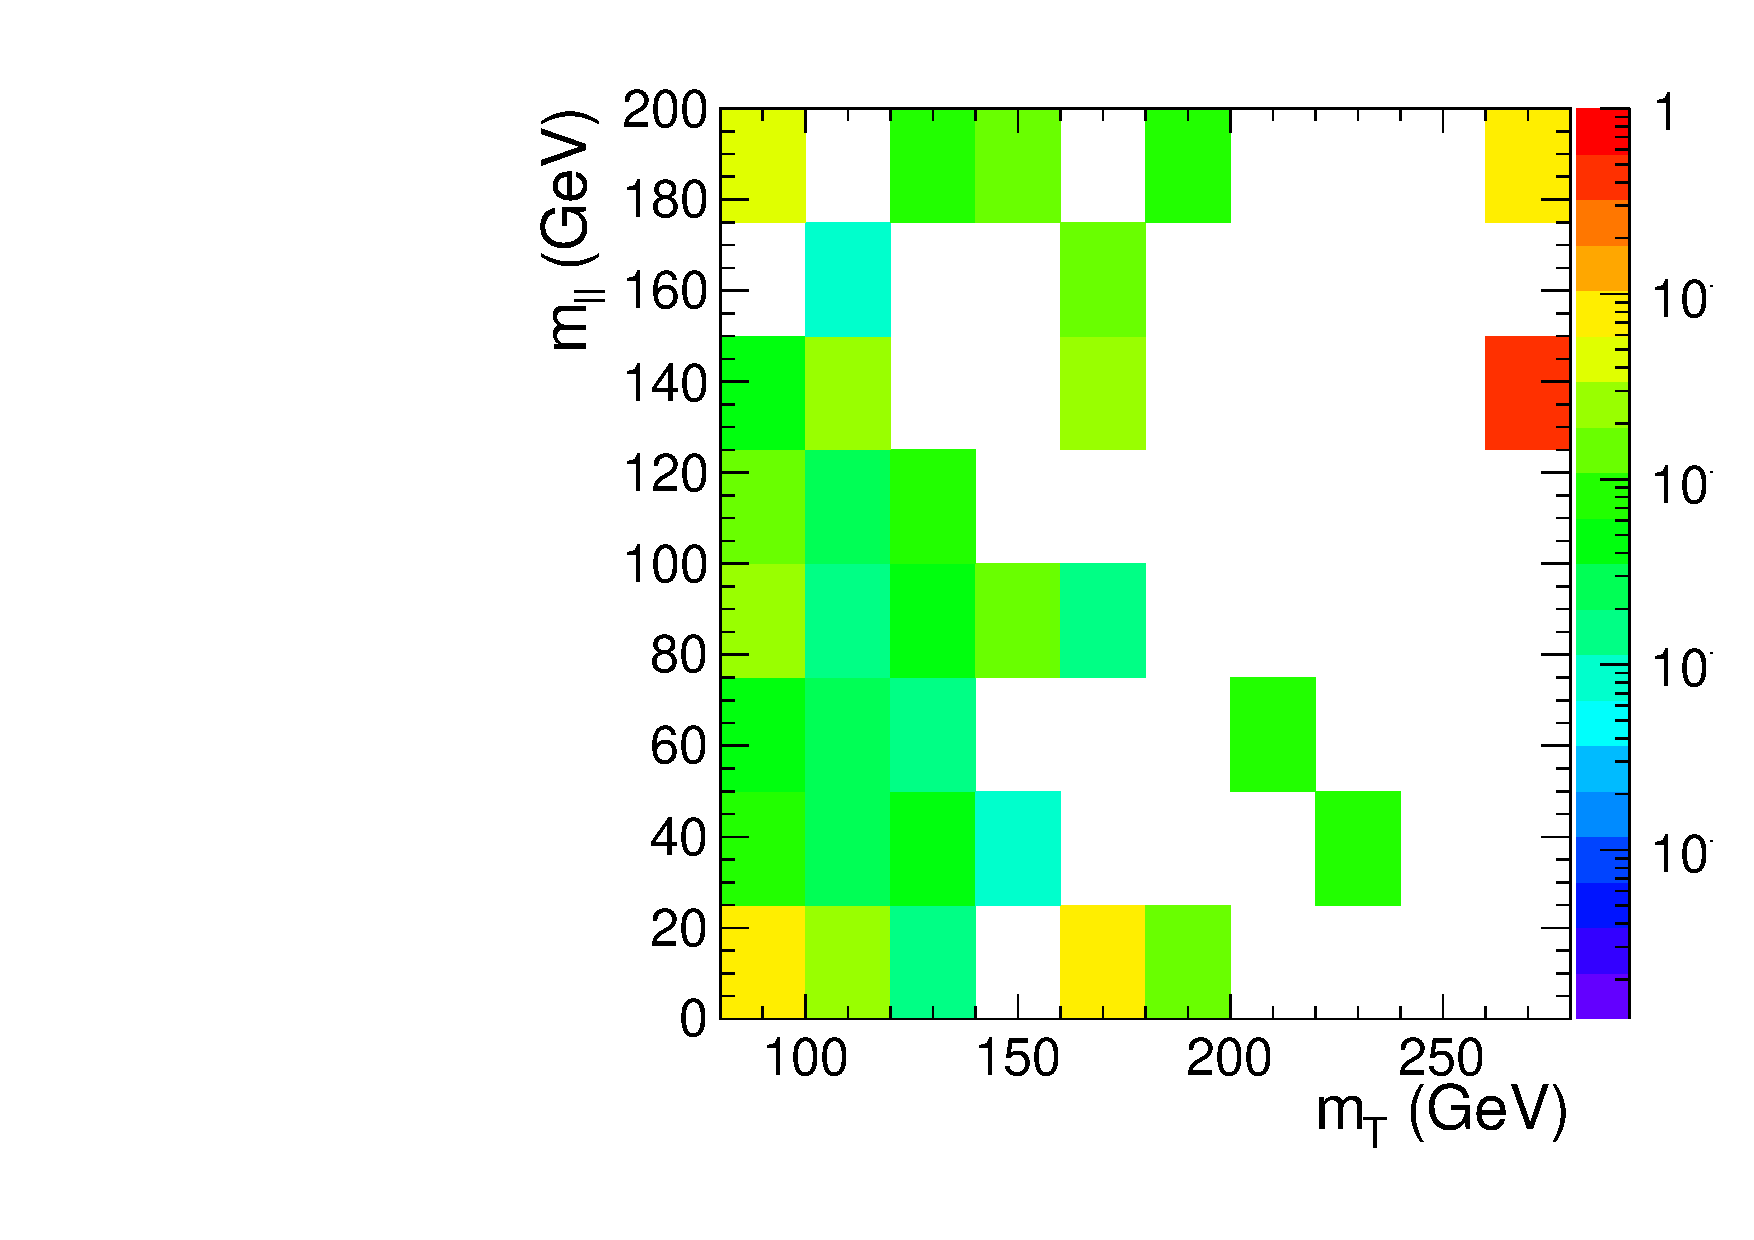
\includegraphics[width=.35\textwidth]{figures/templates/Wgammaerr_2D_mH125_0j_of.pdf}
	}

	\caption{2D templates at \mHi = 125 \GeV} 
	\label{fig:templates_125_3}

\end{figure} 

\begin{figure}[!hbtp]
	
	%
	\centering
	\subfigure[Stacked unrolled template linear]{
	\centering
	\label{subfig:template_unroll_stack_lin}
		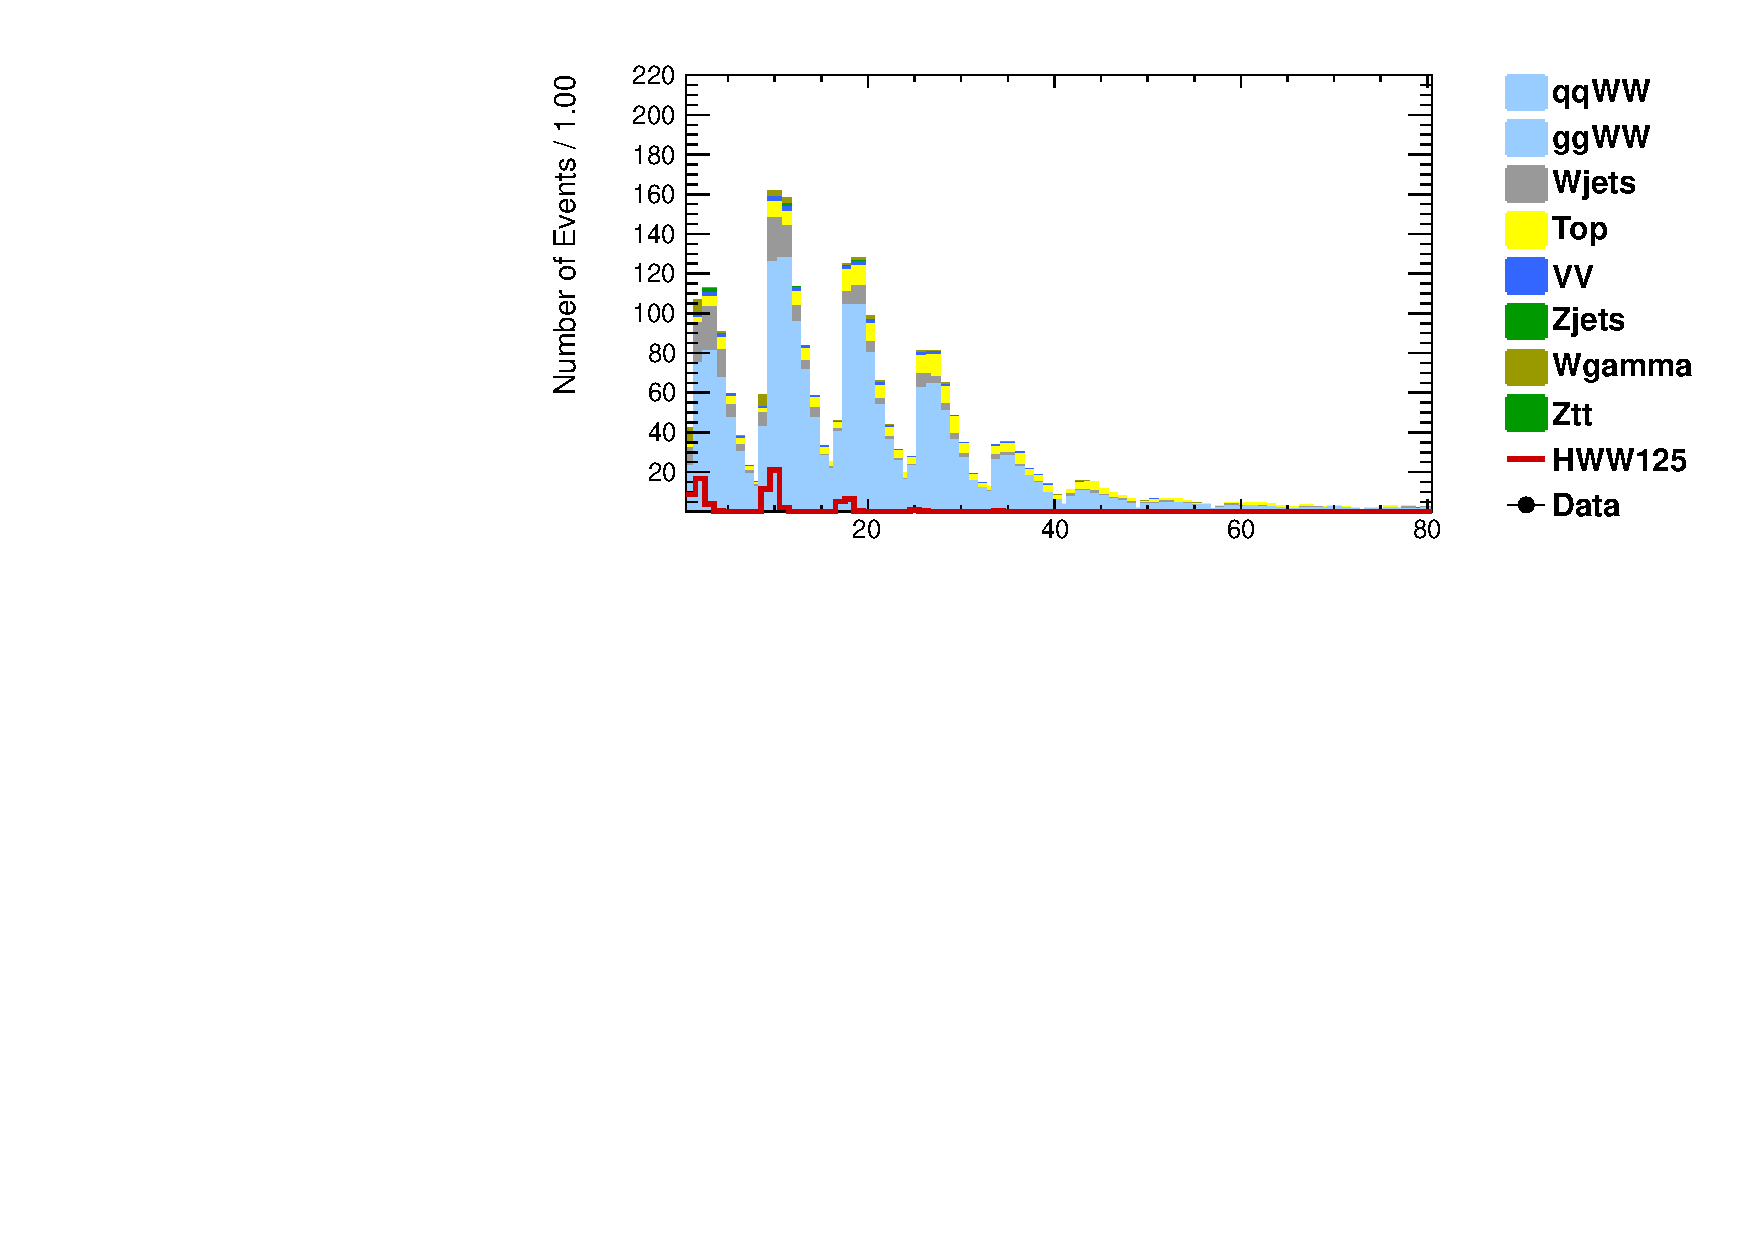
\includegraphics[width=.45\textwidth]{figures/templates/2D_mH125_0j_of_stack_lin.pdf}
	}
	\subfigure[Overlaid unrolled template linear]{
	\centering
	\label{subfig:template_unroll_overlay_lin}
		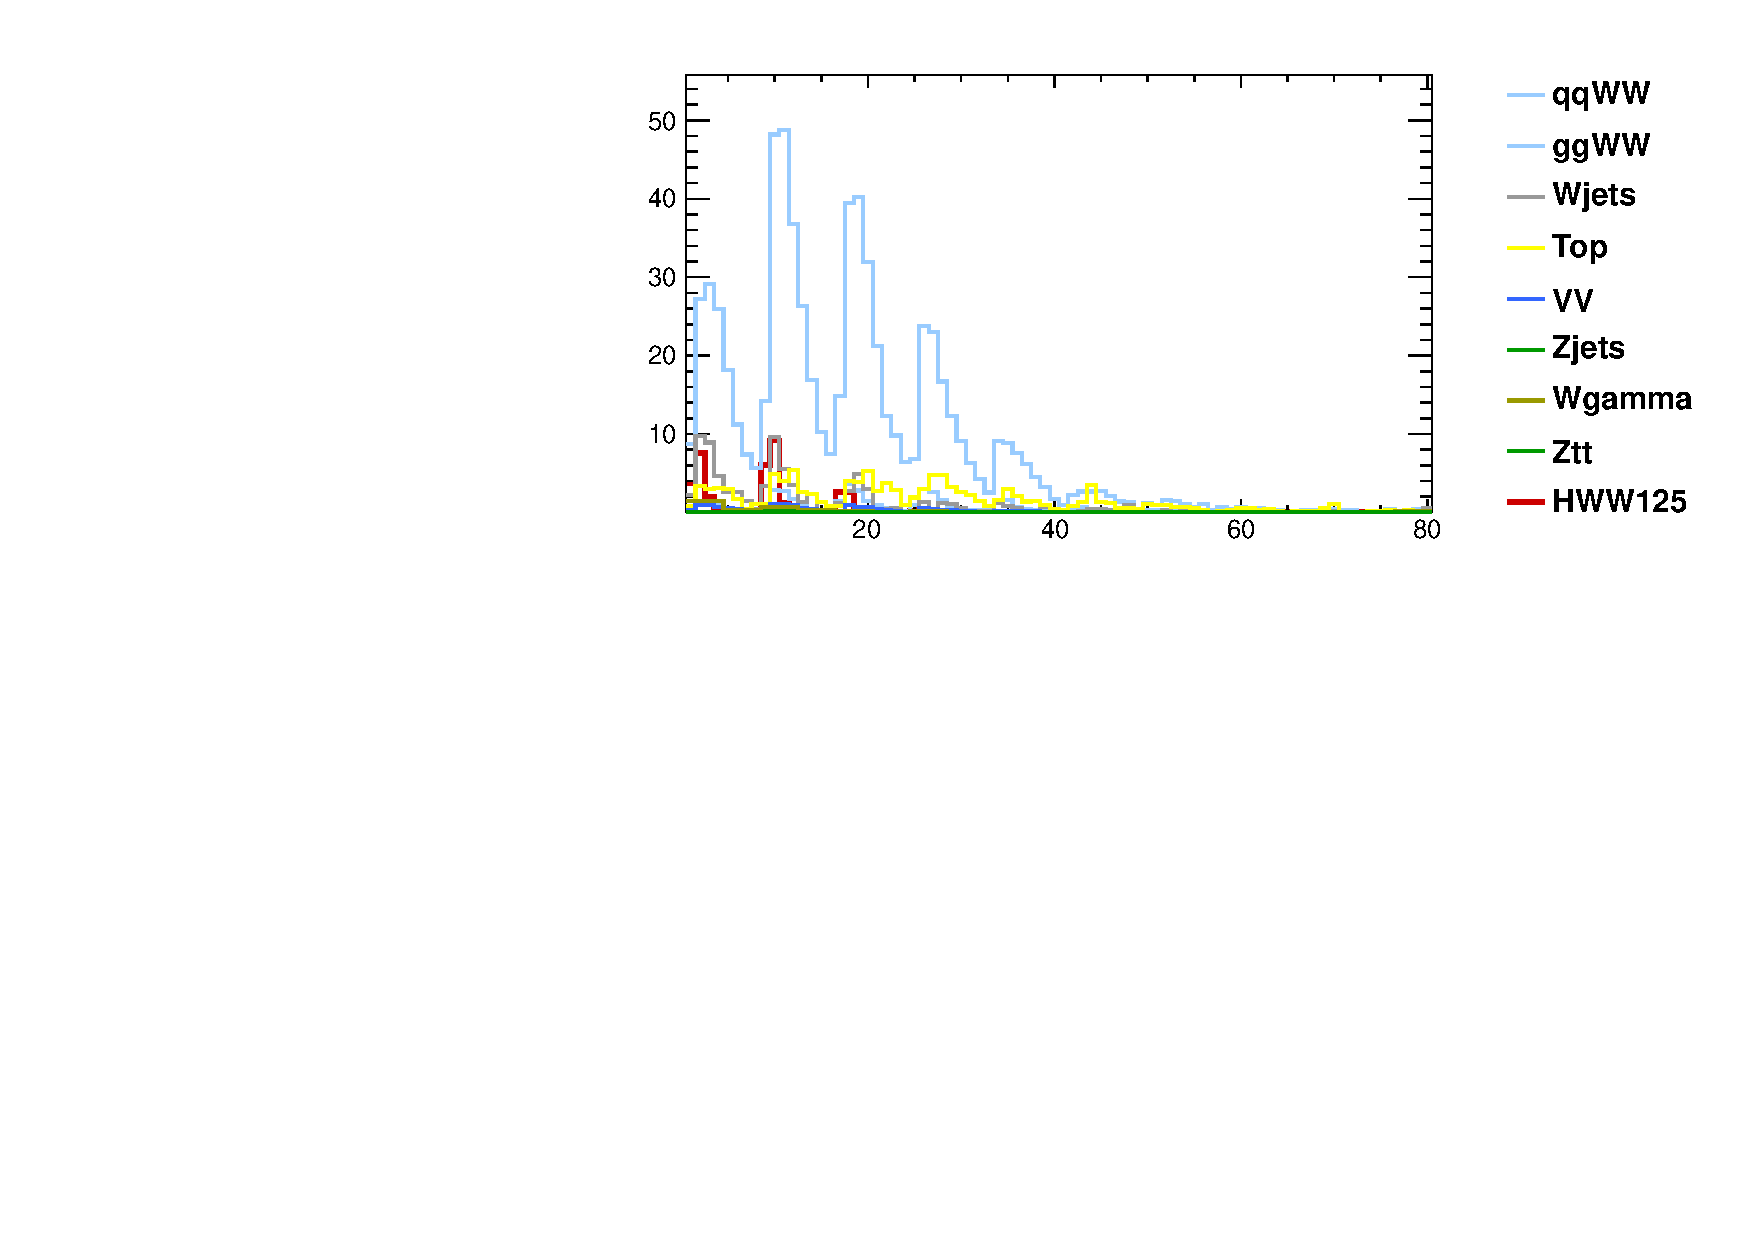
\includegraphics[width=.45\textwidth]{figures/templates/2D_mH125_0j_of_overlay_lin.pdf}
	}

	%
	\centering
	\subfigure[Stacked unrolled template in log scale]{
	\centering
	\label{subfig:template_unroll_stack_log}
		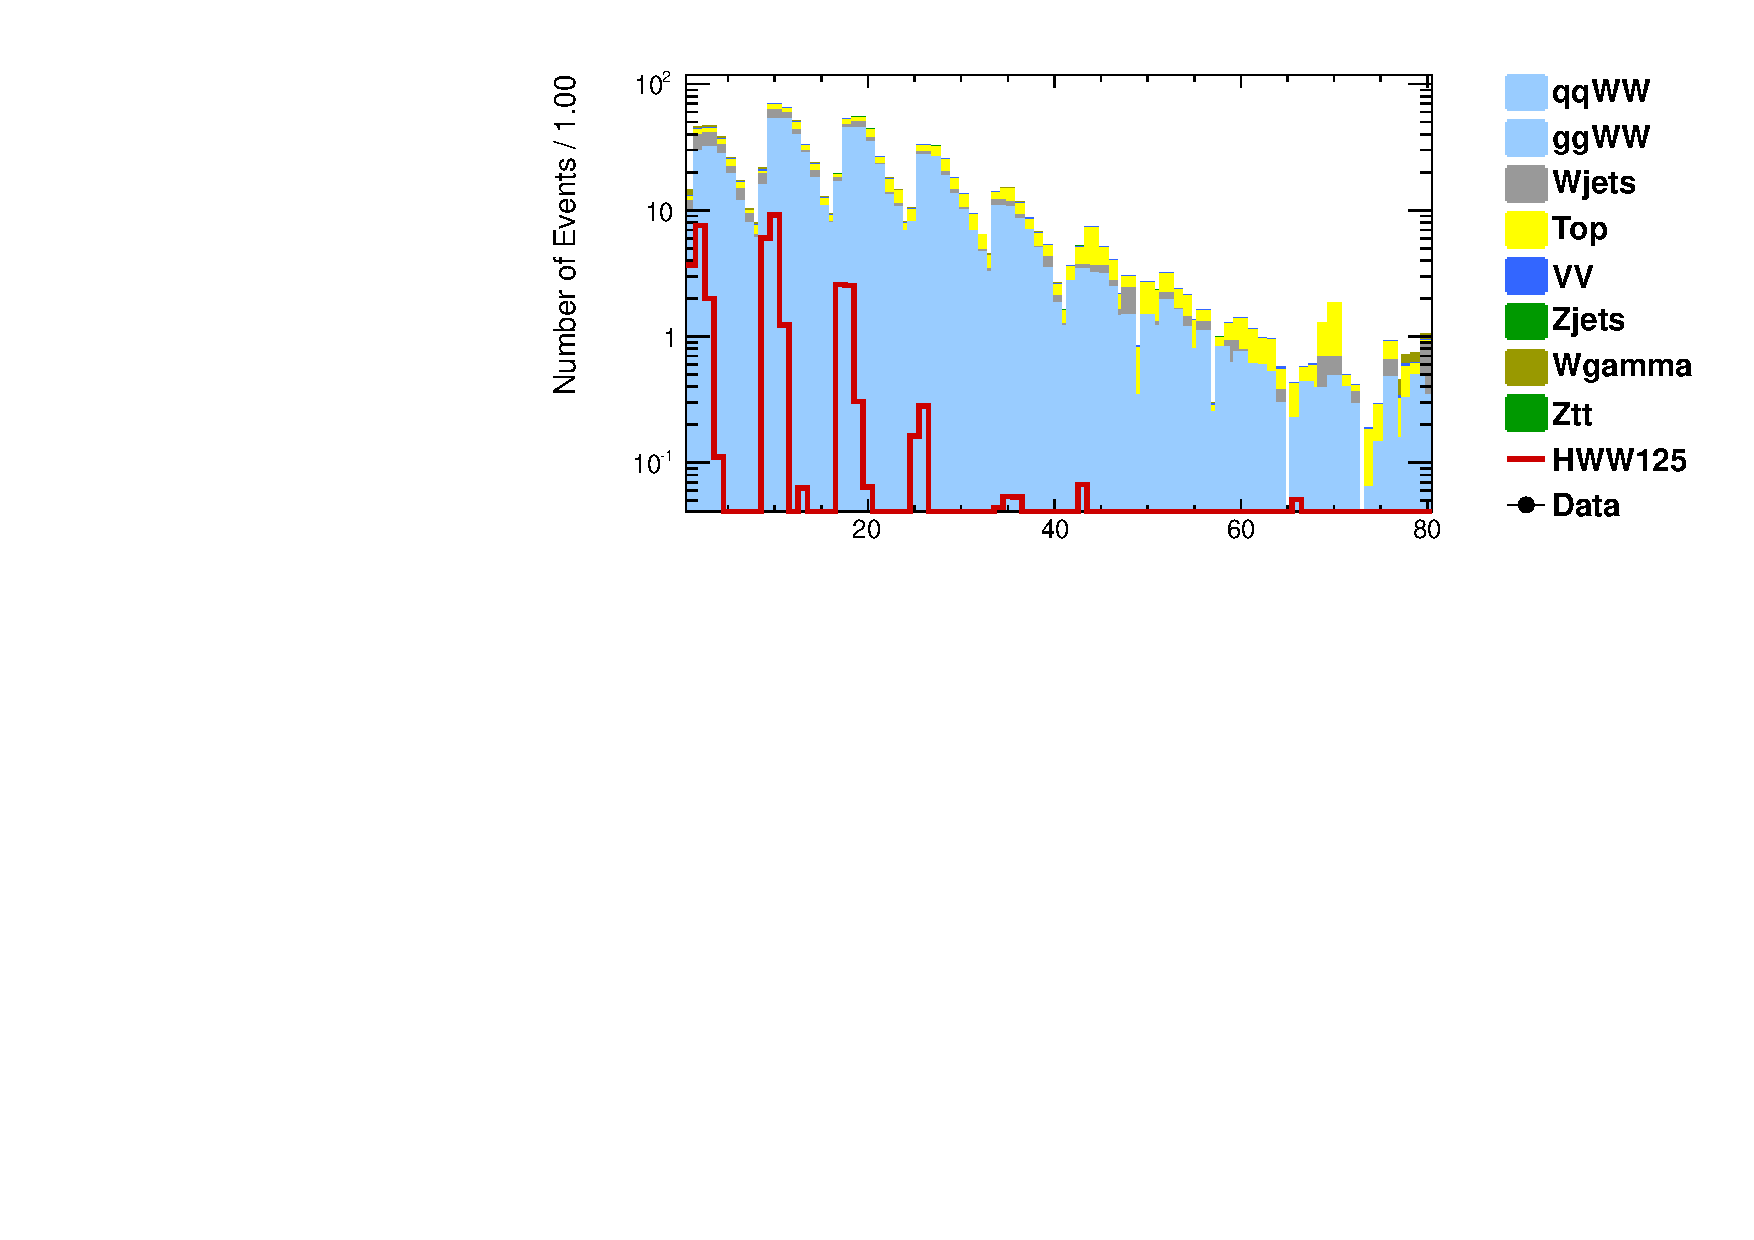
\includegraphics[width=.45\textwidth]{figures/templates/2D_mH125_0j_of_stack_log.pdf}
	}
	\subfigure[Overlaid unrolled template in log scale]{
	\centering
	\label{subfig:template_unroll_overlay_log}
		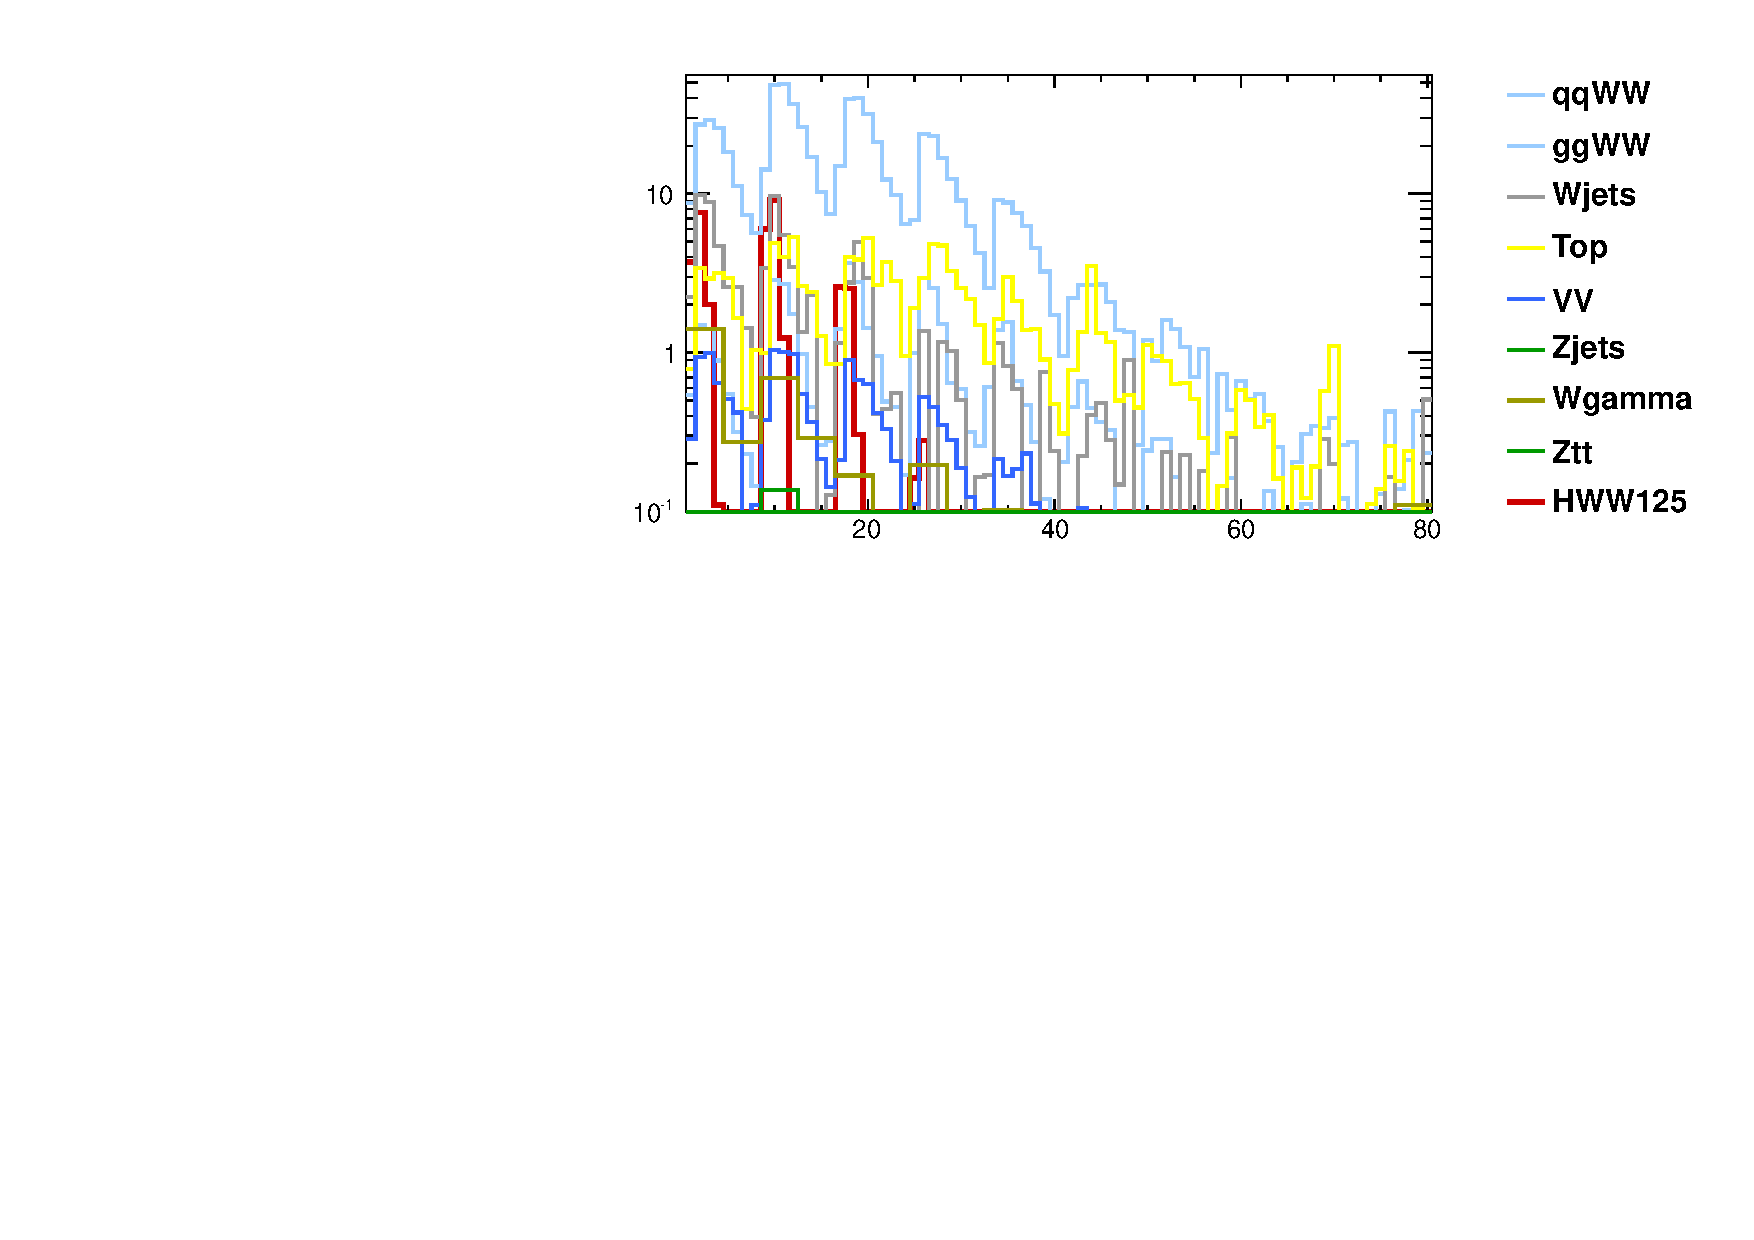
\includegraphics[width=.45\textwidth]{figures/templates/2D_mH125_0j_of_overlay_log.pdf}
	}

	\caption{Unrolled templates at \mHi = 125 \GeV} 
	\label{fig:templates_125_unroll}

\end{figure} 


Figures \ref{fig:templates_125_1} - \ref{fig:templates_125_3} show 2D templates(left) and 
its statistical uncertainties(right) at \mHi = 125 \GeV. The statistical uncertainties 
are relative to the total background yields. Templates for \mHi = 160 \GeV~and 200 \GeV~
are shown in appendix ~\ref{app:templates_160_200}.
